% MSc dissertation example file, February 2022
%
% Leave one of the documentclass lines uncommented to match your degree.
% You may remove the logo option if it causes problems.
% Do not change any other options.
% \documentclass[logo,msc,adi]{infthesis}     % Adv Design Inf
% \documentclass[logo,msc,ai]{infthesis}      % AI
% \documentclass[logo,msc,cogsci]{infthesis}  % Cognitive Sci
\documentclass[logo,msc,cs]{infthesis}      % Computer Sci
% \documentclass[logo,msc,cyber]{infthesis}   % Cyber Sec
% \documentclass[logo,msc,datasci]{infthesis} % Data Sci
% \documentclass[logo,msc,di]{infthesis}      % Design Inf
% \documentclass[logo,msc,dsti]{infthesis}    % Data Sci TI
% \documentclass[logo,msc,inf]{infthesis}     % Informatics
%\documentclass[logo,msc]{infthesis}           % degree unspecified, do not change except to add your degree
%%%%%%%%%%%%%%%%%%%%%%%%
% Understand any problems and seek approval before assuming it's ok to remove ugcheck.
\usepackage{msccheck}
% Include any packages you need below, but don't include any that change the page
% layout or style of the dissertation. By including the ugcheck package above,
% you should catch most accidental changes of page layout though.
\usepackage{microtype} % recommended, but you can remove if it causes problems
\usepackage[authoryear]{natbib}
\usepackage{graphicx}
\usepackage{amsmath}
\usepackage[hidelinks]{hyperref}   
\usepackage{float}
\usepackage{tabularx}
\begin{document}
\begin{preliminary}
\title{Small Language Models for AI-Generated Text Detection: A Comparative Analysis of Curvature Methods}
\author{Royceton Yeoh Tze Jian}
\date{\today}
\abstract{
Text written by large language models now passes for human writing at a scale that no human review team can match, yet the tools built to catch it are too expensive to run where they are most needed. This dissertation asks whether a promising family of detectors, which needs no training data and no access to the suspect model, can instead run on ordinary consumer hardware. These detectors work by editing a document slightly and watching how a language model's confidence in it changes: machine-written text sits on a peak of the model's confidence, so small edits make the confidence fall sharply, whilst human text barely moves. The standard recipe for this test is expensive, because it uses one large model to score the text and a second large model to write the edits. Four controlled experiments show that this expense is not essential. Smaller scoring models detect better than larger ones, partially trained copies of a model detect better than finished ones, and the edits do not need to make sense at all: replacing words at random works as well as, or better than, careful rewriting. The explanation is that detection depends on how sharply the scoring model's confidence changes near the text, and small, unfinished models change most sharply. The pipeline therefore compresses to a detector small enough for a phone, with little loss of accuracy. Within the scope tested (one English corpus, no training), this makes the method practical for on-device use.
}
\maketitle
\newenvironment{ethics}
{\begin{frontenv}{Research Ethics Approval}{\LARGE}}
{\end{frontenv}
\newpage}
\begin{ethics}
This project was planned in accordance with the Informatics Research
Ethics policy. It did not involve any aspects that required approval
from the Informatics Research Ethics committee.
\standarddeclaration
\end{ethics}
\begin{acknowledgements}
I extend my deepest gratitude to my supervisor, Rik Sarkar, for his invaluable tutelage, insightful feedback, and steadfast support throughout this research. I am also profoundly grateful to my parents, whose constant encouragement made this work possible.
\end{acknowledgements}
\tableofcontents
\end{preliminary}

\chapter{Introduction}
\label{chap:introduction}
A language model is a program trained to predict text, and the largest of these programs now write articles, emails and essays that readers struggle to tell apart from human writing \citep{crothers2023machine}. The same capability enables plagiarism, disinformation and abuse at a scale no human review team can match, which creates demand for detectors that can tell whether a document was written by a person or by a model. In this dissertation the model that wrote the suspect text is called the generator, and the model that scores a document is called the detector.
Existing detectors fall into three families, and each fails in a different way. Supervised classifiers are trained on labelled examples of human and machine text, but they memorise the habits of the generators they were trained on and collapse when a new generator appears \citep{wu2025survey}. Watermarks ask the generator to embed a secret statistical pattern in its output, but only cooperative generators carry the pattern and simple rewriting removes it \citep{kirchenbauer2023watermark}. The third family, and the subject of this dissertation, needs neither labelled data nor a cooperative generator. These zero-shot methods use any language model as a scorer and decide authenticity from how that model's probabilities behave \citep{mitchell2023detectgpt}.
The specific method studied here is probability curvature \citep{mitchell2023detectgpt}. Every language model assigns a number to a text, its log probability, which records how likely the model considers the text. The method makes many small edits to the document, called perturbations, and compares the log probability of the original with the average log probability of the edited copies; the difference is the curvature score. A generator writes the text it considers most likely, so machine-written text sits at a peak of the scorer's log probability and most edits lower that value, giving a large positive score. Human text sits on flatter ground, where edits raise or lower the value at random, giving a score near zero. A document is flagged as machine-written when its score is positive and large.
The method is accurate but expensive as usually implemented. The scorer is normally a large language model, and the perturbations are normally written by a second large model that fills in masked blanks, so one document costs dozens of passes through two large models. That cost rules out the places detection is most needed, namely phones, browser extensions and small local servers, collectively called edge devices, where memory and battery are scarce and sending text to a cloud service raises privacy concerns.
This dissertation argues that the expense is an artefact of the usual implementation, not of the method. The detection signal lives in how sharply the scorer's log probability changes when the text is edited, and that sharpness is strongest in small, partially trained models. Four controlled experiments support this claim. Detectors as small as Pythia-70M and DistilGPT-2, with 70 to 82 million parameters, separate human from machine text with an AUROC above 0.90 against the majority of 13 unseen generators, where AUROC is a standard score in which 1.0 is perfect and 0.5 is a coin flip, whilst detectors of 1.5 to 1.7 billion parameters frequently perform no better than the coin flip. Copies of a detector saved early in training, called checkpoints, outperform the finished model, with an optimal window between 1,000 and 10,000 steps. The model that writes the perturbations shows diminishing returns beyond a medium size. Most strikingly, the perturbations need not make sense: replacing words uniformly at random works as well as, or better than, careful rewriting. The cheapest correct implementation of the pipeline is therefore among the strongest.
Stated precisely, the problem is to determine which constituents of the curvature pipeline govern the separability of the curvature score between human and machine text, and whether each constituent can be replaced by a cheaper alternative without collapsing that separability. Formally, for a text $x$ scored by a detector $\theta$, the curvature score is denoted as $z(x) = \log p_\theta(x) - \frac{1}{n}\sum_{i=1}^{n} \log p_\theta(x_i)$, and machine text is flagged when $z(x)$ is positive and large (Equation~\ref{eq:curvature}). The question is not trivial, because the four constituents (detector scale, training state, perturbation-model capacity and perturbation semantics) interact, and a naive cost-cut could destroy the very signal the method relies upon. Figure~\ref{fig:pipeline} summarises the pipeline that all four experiments share, and Figure~\ref{fig:exp1_scale_trend} previews the central empirical result: mean detection performance declines monotonically as the detector grows, falling below the coin-flip level at 1.7 billion parameters.

\section{Motivation}
\label{sec:motivation}
The motivation is the gap between what detection costs and where it must run. Curvature methods are accurate, but their original form required large models for both scoring and perturbation \citep{mitchell2023detectgpt}. Later work cut part of the cost, for example by drawing the perturbations from the scorer itself instead of a second model \citep{bao2024fast}, and other research explored complementary signals such as writing style \citep{breneur2026notai}, the statistical glue between neighbouring words \citep{ma2024zero}, and implicit reward models \citep{liu2026zero}. Despite these advances, the scoring model is still assumed to be large and fully trained, and a large model cannot run in real time on a phone, a browser extension or an embedded board.
At the same time, there is early evidence that the assumption is backwards: smaller language models can be stronger detectors than larger ones \citep{mireshghallah2023smaller}, because a small model is less certain and its probabilities therefore move more when it meets the statistical fingerprints of machine text. The central aim of this dissertation is to test and explain that observation, and to turn it into a practical recipe for on-device detection.

\section{Research Objective}
\label{sec:research_objective}
This dissertation seeks to isolate the precise variables that enable curvature-based detection by systematically modifying key components of the detection pipeline. The central questions guiding this dissertation include:
\begin{itemize}
\item How does the detector's parameter count influence detection across generators, and do smaller models truly provide superior cross-detection than larger, more confident architectures?
\item How do training checkpoints affect detection, and do partially trained models retain sharper likelihood surfaces before overfitting occurs?
\item Is the capacity of the perturbation model critical, or are compact configurations sufficient compared with massive ones?
\item What are the minimum linguistic and statistical requirements for the curvature metric to work, and how does efficacy vary from meaning-preserving edits to pure token noise?
\end{itemize}

\section{Contributions and Outcomes}
\label{sec:contributions}
This dissertation offers a comparative analysis of the mechanics of zero-shot probability curvature for AI-generated text detection, with the aim of making the method light enough for consumer hardware. Its contributions are as follows:
\begin{itemize}
\item \textbf{Smaller detectors are stronger detectors:} across a 13-generator by 17-detector matrix, detection accuracy falls as the detector grows: 70 to 82 million parameter detectors exceed 0.90 AUROC against most unseen generators, whilst billion-parameter detectors fall to chance. Larger detectors assign conservative, smooth likelihoods to out-of-distribution text, whereas smaller models expose sharper probability gradients, generalising the narrower prior observation of \citet{mireshghallah2023smaller}.
\item \textbf{Partial training improves detection:} checkpoints saved between 1,000 and 10,000 training steps outperform the finished model, because intermediate weights retain broad, less specialised probability distributions that have not yet overfit, yielding sharper sensitivity to synthetic text from unseen generators.
\item \textbf{Perturbation capacity obeys diminishing returns:} comparing T5-small, T5-large and T5-3B shows that moving from a small to a medium mask-filler recovers most of the signal whilst a filler twenty times larger adds little, clarifying that the computational overhead of massive mask-filling models is unnecessary for edge deployment.
\item \textbf{Semantic coherence is unnecessary:} the systematic comparison of semantic, synonym, unigram and random-token perturbations shows that uniform random replacement matches or beats careful, meaning-preserving rewriting, isolating the minimum statistical prerequisite of the curvature metric and allowing the second model to be removed entirely.
\end{itemize}
Taken together, these findings compress the pipeline to one small, partially trained detector plus an inexpensive random edit, a configuration that fits in a few hundred megabytes and needs no labelled data, no access to the generator and no cloud. Within the scope tested, this yields a practical, architecture-agnostic path to on-device detection.

\section{Outline}
\label{sec:outline}
This dissertation is organised as follows:
\begin{itemize}
\item \textbf{Chapter \ref{chap:introduction}: Introduction} establishes the motivation, states the central problem and the headline findings up front, and outlines the structure of the dissertation.
\item \textbf{Chapter \ref{chap:background}: Background and Related Work} reviews the evolution of Large Language Models, the current landscape of machine-generated text detection, and the theoretical foundations of loss landscape curvature.
\item \textbf{Chapter \ref{chap:methodology}: Methodology} details the unified experimental framework, curvature formulations, dataset configurations, and evaluation metrics employed across all tests.
\item \textbf{Chapter \ref{chap:exp1}: Experiment 1: Cross-Detection and Model Scale} presents the findings regarding how detector parameter count influences cross-architecture generalisation.
\item \textbf{Chapter \ref{chap:exp2}: Experiment 2: Training Checkpoint Dynamics} examines how the evolution of detector weights over time affects the sharpness of the likelihood surface.
\item \textbf{Chapter \ref{chap:exp3}: Experiment 3: Semantic Perturbation Scale} evaluates the impact of the mask-filling model capacity on the accuracy of the curvature metric.
\item \textbf{Chapter \ref{chap:exp4}: Experiment 4: Linguistic Perturbation Strategies} tests the minimum statistical and semantic prerequisites required to probe the loss landscape effectively.
\item \textbf{Chapter \ref{chap:conclusion}: Conclusion} synthesises the key findings of the four experiments with a focus on the practical viability of deploying Small Language Models on edge devices, acknowledges the limitations of this dissertation, and proposes avenues for future research.
\end{itemize}

\chapter{Background and Related Work}
\label{chap:background}
Machine-generated text is difficult to detect because modern generators leave only faint statistical traces. This chapter reviews the prior work that this dissertation builds upon, and it frames each detection paradigm by the failure mode that motivates the next. A reader who is new to the field should finish the chapter understanding four things: what a language model is and why it made detection hard (Section \ref{sec:llm_evolution}), how the three existing detector families each fail (Section \ref{sec:detection_landscape}), what the curvature metric measures (Section \ref{sec:zero_shot}), and why small models are the promising detectors (Section \ref{sec:slm}).

\section{How Large Language Models Created the Detection Problem}
\label{sec:llm_evolution}
A language model is a program trained to predict the next word of a text; run repeatedly, it can write whole documents. Modern text generators descend from two architectural lineages. Recurrent networks, such as long short-term memory networks, processed text one word at a time, so they captured local dependencies but trained slowly and struggled with long contexts \citep{hochreiter1997long, vinyals2015neural}. The Transformer replaced word-by-word processing with self-attention, a mechanism that lets every word look at every other word in one step, which parallelised training and unlocked much longer contexts \citep{vaswani2017attention}. Successive releases, from GPT-2 to the OPT and GPT-Neo families, scaled these architectures by orders of magnitude \citep{radford2019language, zhang2022opt, black2021gpt}. Scaling laws made the resulting growth predictable: test loss, the model's error on unseen text, falls smoothly as parameters, data and compute grow \citep{kaplan2020scaling, hoffmann2022training}.
Scale brought fluency. Contemporary generators produce text that human readers struggle to separate from human writing, and the surface artefacts that early detectors exploited, such as repetition and unnatural word choice, have largely disappeared. Detection therefore has to look below surface fluency, at the statistics of the generator itself. The next section reviews the three detection paradigms and the failure mode of each.

\section{Detection Paradigms and Their Failure Modes}
\label{sec:detection_landscape}
Three families of detectors dominate the literature: supervised classifiers, watermarks and zero-shot statistical tests. A supervised classifier learns from labelled examples, a watermark is a hidden pattern embedded by the generator, and a zero-shot test needs neither examples nor cooperation. Each family solves part of the problem, and each fails in a way that motivates the next family.

\subsection{Supervised Classification and the Generalisation Failure}
\label{sec:supervised}
Supervised detectors train a classifier on labelled human and machine text, usually by fine-tuning, that is, continuing the training of, a pre-trained encoder, a model that reads text and produces a numerical summary of it. Early systems exploited rank-based statistics of generated text, as in the GLTR analysis tool, which flags text whose words are unusually predictable \citep{gehrmann2019gltr}, and later systems such as GROVER showed that a large model can discriminate synthetic articles from real ones \citep{zellers2019defending}. Accuracy is high whenever the test generator appears in the training set.
Generalisation is the failure mode. Benchmarks such as MGTBench show that supervised detectors lose most of their accuracy once the test generator is unseen \citep{he2024mgtbench}. The classifier memorises the quirks of its training generators rather than a universal signature of synthesis, so every new generator demands fresh labels and a round of retraining \citep{crothers2023machine, wu2025survey}. A detector that must be retrained for every new generator cannot keep pace with the open-ended stream of new models.

\newpage
\subsection{Watermarking and the Coverage Failure}
\label{sec:watermarking}
Watermarking moves the burden to the generator. At each step, the generator partitions its vocabulary into a secret green list of preferred words and biases sampling towards that list, embedding a statistical signature that a verifier who knows the secret can later test \citep{kirchenbauer2023watermark}. Later work scaled the idea to larger models and open-ended sampling \citep{dathathri2024scalable}. Detection is near-perfect on watermarked text and needs no labelled data.
Coverage is the failure mode. A watermark binds only the generators that adopt it, so open-weight models and proprietary black boxes remain unwatermarked and undetectable by this route. Paraphrase, translation and synonym replacement also strip the signature while preserving meaning \citep{kirchenbauer2023watermark}. Watermarking is therefore a provenance mechanism for cooperative generators, not a general detector.

\section{Zero-Shot Detection and Probability Curvature}
\label{sec:zero_shot}
Zero-shot detectors remove the need for labels and for generator cooperation. Zero-shot means the detector is used as-is, with no training examples of the text it must judge. Such detectors test a document against the probability landscape of an arbitrary language model, and they decide authenticity from the geometry of that landscape alone \citep{sadasivan2023can}. The most influential method in this family is DetectGPT \citep{mitchell2023detectgpt}.
The key idea is curvature. Every language model assigns a number to a text, its log probability, which records how likely the model considers the text; let $\log p_\theta(x)$ denote this value for a detector $\theta$ and a text $x$. Machine-generated text sits near a local maximum of this surface, because the generator concentrates its mass on the sequences it is most likely to produce. Small perturbations of such a text, that is, small edits, move it off the peak, and the log probability drops. Human text sits on flatter ground, where perturbations move the log probability up or down with no consistent direction. Figure \ref{fig:curvature_concept} illustrates this asymmetry, and Equation \ref{eq:curvature} in Chapter \ref{chap:methodology} formalises it: the curvature of $x$ is the difference between $\log p_\theta(x)$ and the mean log probability of its perturbed neighbours.
\begin{figure}[H]
\centering
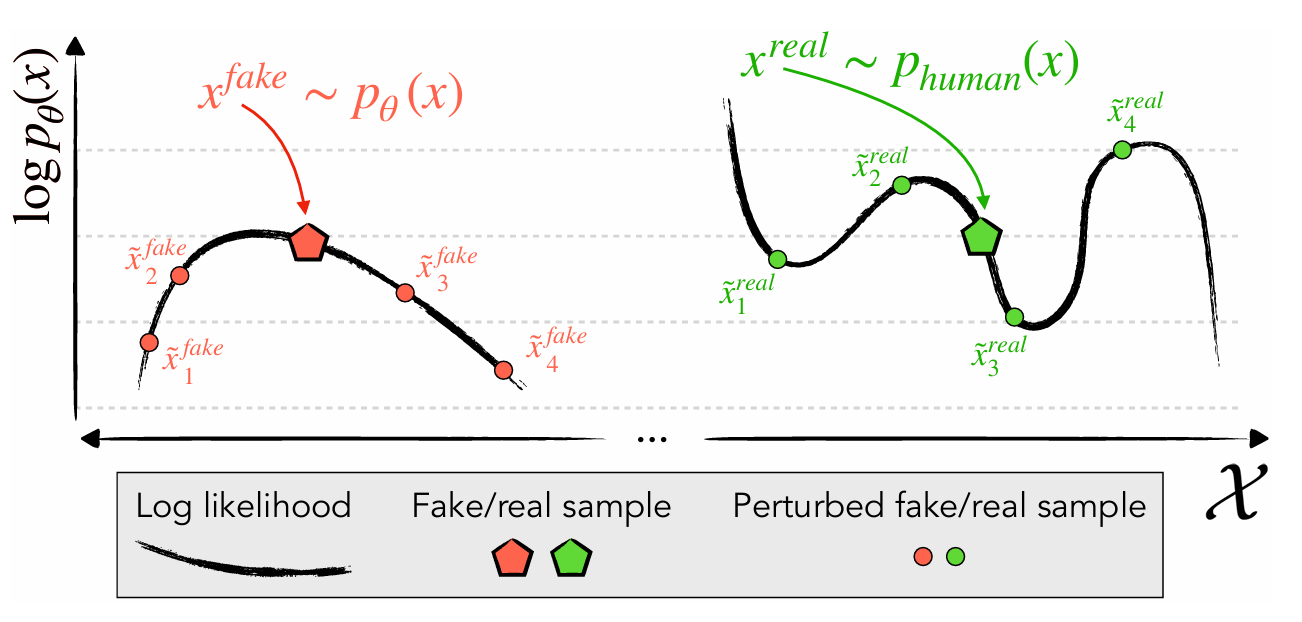
\includegraphics[width=\textwidth]{figures/Background/detectgpt_curvature.png}
\caption{Probability curvature in the log probability landscape. Left: machine-generated text occupies a region of negative curvature, where most perturbations lower the log probability on average. Right: human-written text sits on flatter ground, where perturbations move the log probability up or down with no consistent direction. Adapted from Mitchell et al. (2023).}
\label{fig:curvature_concept}
\end{figure}
DetectGPT instantiates the perturbations with a masked language model, typically from the T5 family, that rewrites the masked spans, in other words a second model hired to fill in the blanks \citep{raffel2020exploring}. This perturbation step is the bottleneck: every document requires dozens of mask-filling passes through a large model. Fast-DetectGPT replaces mask-filling with conditional sampling, drawing the edits from the detector itself, and cuts the cost sharply \citep{bao2024fast}. Other zero-shot tests use different statistical signals, such as the cross-model agreement used by Binoculars, which compares two models' opinions of the same text \citep{hans2024spotting}, yet they all share the same premise: the geometry of model probabilities carries a signature of synthesis.
Two questions remain open, and they define this dissertation. First, any model can in principle serve as the scoring model, so which model properties make a good detector? Second, how much of the perturbation machinery is truly necessary? The next section reviews the evidence that smaller models answer the first question.

\newpage
\section{Small Language Models as Edge Detectors}
\label{sec:slm}
Small language models occupy the lower end of the scaling spectrum, with parameter counts from roughly 70 million to 3 billion. The Pythia suite is the salient resource for studying them: it releases decoder-only Transformers, models that generate text one token at a time, from 70 million to 12 billion parameters, trained on identical data with identical hyperparameters, and it publishes 154 checkpoints, saved copies of the model taken during training, per model \citep{biderman2023pythia}. The SmolLM family pushes efficiency further whilst retaining competitive language modelling \citep{allal2024smollm}. GPT-2 and its distilled variant DistilGPT-2, a smaller model trained to imitate the larger one, remain standard baselines with well-characterised training dynamics \citep{radford2019language, sanh2019distilbert}.
Edge deployment is the practical stake. An edge device is a consumer product such as a phone, a browser extension or an embedded board, where memory, battery and bandwidth are scarce. A detector that fits in a few hundred megabytes can run on such a device with no cloud round-trip and no privacy cost. Large detectors cannot meet these constraints. Prior work has established that small language models can be stronger zero-shot detectors than large ones \citep{mireshghallah2023smaller}, but that evidence covers only a narrow set of generator and detector pairs, and it leaves three questions unanswered. First, no study has traced how detector scale interacts with cross-architecture generalisation across a broad generator suite. Second, no study has traced how the training checkpoint, as opposed to the parameter count, shapes the curvature signal. Third, no study has isolated whether the semantic coherence of the perturbation, as opposed to its statistical disruption, matters at all. These three gaps, together with the scale question, define the four experiments of this dissertation.

\section{Chapter Summary}
\label{sec:background_summary}
This chapter has reviewed the three detection paradigms and their failure modes: supervised classifiers fail to generalise, watermarks fail to cover, and zero-shot curvature methods remain computationally heavy. It has introduced the curvature metric and the evidence that smaller models are sharper detectors. The following chapter, Chapter \ref{chap:methodology}, defines the unified framework, the dataset, the metrics and the curvature formulation used in the four experiments.

\chapter{Methodology}
\label{chap:methodology}
This chapter details the unified experimental framework used to conduct the comparative analysis of curvature-based detection. Recall from Chapter \ref{chap:background} that the method scores a document, makes many small edits to it, and compares the detector's confidence in the original and in the edits. The pipeline has four constituents that can be varied: the detector, the language model that scores the text; its training state, the point in training at which the detector's weights are frozen; the mask-filler, the second model that writes the edits; and the editing strategy, the rule used to produce those edits. Figure \ref{fig:pipeline} summarises the pipeline that all four experiments share. Table \ref{tab:perturbation_example} provides a worked example of the editing strategies, and Table \ref{tab:design} summarises how each experiment varies exactly one constituent. Section \ref{sec:dataset} describes the dataset, Section \ref{sec:metrics} defines the evaluation metrics, Section \ref{sec:curvature_formulation} presents the curvature formulation, Section \ref{sec:perturbations} details the perturbation strategies, and Section \ref{sec:experimental_design} details the experimental design.
\begin{figure}[H]
\centering
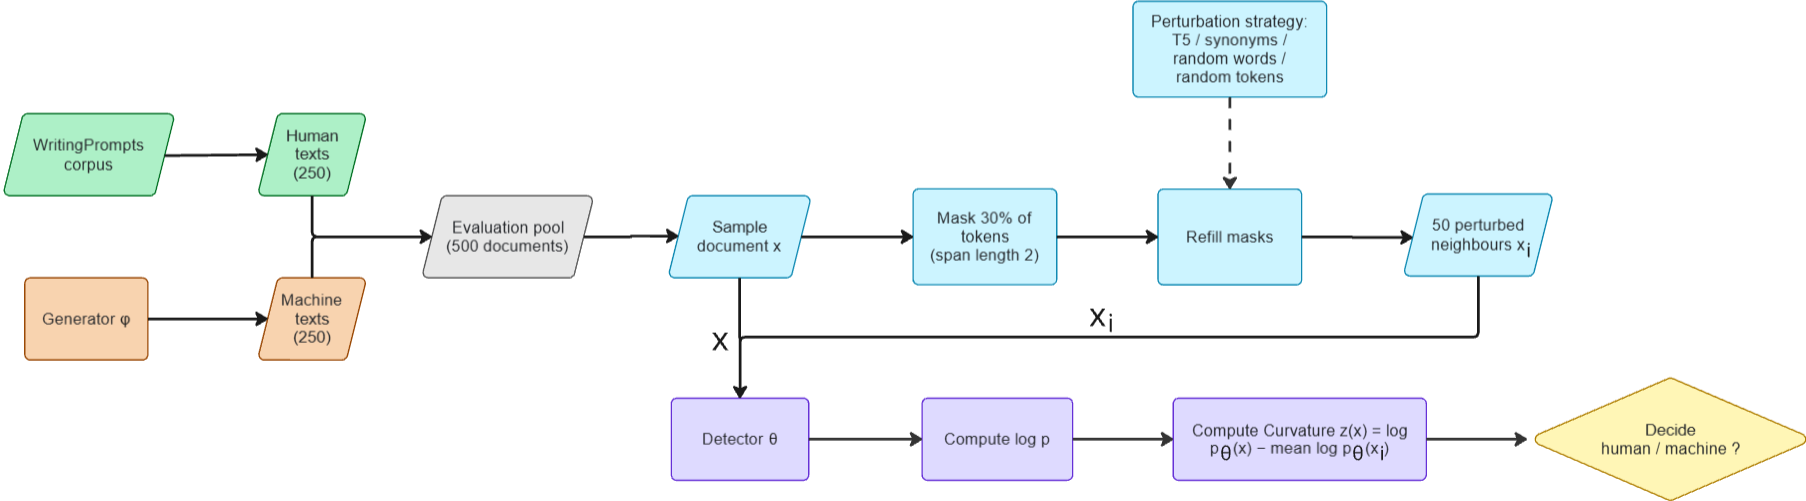
\includegraphics[width=0.85\textwidth]{figures/Methodology/pipeline_diagram.png}
\caption{The unified curvature-based detection pipeline. Human (WritingPrompts) and machine texts from a generator $\phi$ form a balanced 500-document pool. A sampled document $x$ is masked (30\% of tokens in two-token spans) and refilled via a chosen strategy (dashed arrow) to yield 50 perturbed neighbours $x_i$. Detector $\theta$ scores $x$ and $x_i$, and the curvature $z(x) = \log p_\theta(x) - \overline{\log p_\theta(x_i)}$ is thresholded into a decision. Each experiment varies one component while holding the rest fixed.}
\label{fig:pipeline}
\end{figure}

\section{Dataset Configuration}
\label{sec:dataset}
The evaluation dataset for all experiments is sourced from the WritingPrompts corpus \citep{fan2018hierarchical}, a public collection of human-written creative stories, each prompted by a one-line premise. The corpus provides a diverse array of linguistic styles, genres and syntactic structures, so the detectors are evaluated on natural, unconstrained human text rather than on highly structured or domain-specific writing, which is critical for assessing the generalisation of zero-shot detectors.
For each generator $\phi$, the model that wrote the machine text, a controlled and balanced pool of 250 human-written samples and 250 machine-generated samples is extracted, giving a 500-document evaluation pool per generator (Figure \ref{fig:pipeline}). The machine-generated samples are produced by a diverse suite of generative models, ensuring a broad representation of synthetic text. The balanced pool removes confounding bias from unbalanced class distributions, so the evaluation metrics reflect the true discriminative capability of the detector rather than its sensitivity to class priors, and any observed variation in performance is attributable to the manipulated constituents rather than to fluctuations in data quality or volume.

\section{Evaluation Metrics}
\label{sec:metrics}
The core metrics for evaluation across all experiments are the Area Under the Receiver Operating Characteristic Curve (AUROC) and the Precision-Recall Area Under the Curve (PR-AUC). Both are threshold-independent scores between 0 and 1, where 1 is perfect separation and 0.5 is no better than a coin flip on this balanced dataset. They therefore give a holistic view of detector performance across all possible classification boundaries.
The AUROC measures the ability of a detector to distinguish human-written from machine-generated text. It is the probability that a randomly drawn machine document outscores a randomly drawn human document, and it plots the True Positive Rate (the proportion of machine text correctly identified) against the False Positive Rate (the proportion of human text incorrectly flagged) at various thresholds. The AUROC is selected for its robustness in assessing cross-architecture generalisation, because it evaluates the ranking quality of the detector scores independently of any fixed decision boundary. A higher AUROC indicates that the detector consistently assigns higher curvature scores to machine text than to human text.
Complementing this, the PR-AUC provides a more stringent evaluation of forensic reliability. It plots Precision (the proportion of flagged text that is actually machine-generated) against Recall (the proportion of machine text that is successfully flagged). In real detection scenarios, minimising false positives on human text is critical, because incorrectly flagging human writing has severe consequences for digital trust and content moderation. Unlike the AUROC, which can remain deceptively high under class imbalance, the PR-AUC is highly sensitive to performance on the positive class. Together, the two metrics give a comprehensive view of detection efficacy.

\section{Curvature Formulation}
\label{sec:curvature_formulation}
The detection mechanism estimates the probability curvature of a text within the log probability landscape of a detector $\theta$. The log probability $\log p_\theta(x)$, introduced in Chapter \ref{chap:background}, is the number that records how likely the detector considers a text $x$. Following Mitchell et al. \citep{mitchell2023detectgpt}, the curvature is approximated by the difference in log probabilities between the original text and its perturbed variants, that is, its edited copies.
The premise is the geometry of neural network loss landscapes. Generated sequences often reside in sharp, high-curvature minima compared with the flatter, more stable regions occupied by human text \citep{li2018visualizing}. In a sharp minimum, minor perturbations to the input produce a steep drop in the model's assigned log probability. In a flat region, perturbations produce minimal change.
Formally, for a text $x$, the detector computes $\log p_\theta(x)$. A set of perturbed sequences $\{x_1, x_2, ..., x_n\}$ is then generated by applying local semantic or statistical edits to the original. The curvature score $z(x)$ is the average log probability difference between the original and its perturbed neighbours:
\begin{equation}
\label{eq:curvature}
z(x) = \log p_\theta(x) - \frac{1}{n} \sum_{i=1}^{n} \log p_\theta(x_i)
\end{equation}
A positive curvature value indicates that the original text sits in a sharp minimum, the signature of machine-generated content. Human text typically yields values near zero or negative, reflecting a flatter surface to which the model is less sensitive. This formulation turns the abstract geometry of the loss landscape into a computable scalar, enabling systematic evaluation of authenticity. All experiments report this raw mean log-likelihood difference, rather than a variant standardised by the perturbation standard deviation, so that curvature scores remain directly comparable across configurations.

\section{Perturbation Strategies}
\label{sec:perturbations}
The perturbation stage constructs the neighbourhood $\{x_i\}$ around each document $x$. Following the masking protocol of DetectGPT \citep{mitchell2023detectgpt}, 30\% of the tokens in each document are masked in spans of length two, that is, pairs of consecutive words are hidden, and $n = 50$ perturbed variants are drawn per sample. Four strategies are compared, spanning a spectrum from full semantic coherence, where the edits keep the meaning, to pure token noise. The semantic control refills the masked spans with a T5 mask-filling model \citep{raffel2020exploring}, a second model trained to fill in blanks. The synonym strategy replaces the spans with lexical substitutes drawn from WordNet \citep{miller1995wordnet}. The random words strategy samples substitutes according to unigram frequency, how often each word appears in the corpus. The random tokens strategy inserts uniformly sampled vocabulary tokens. Table \ref{tab:perturbation_example} illustrates the four strategies on a single document, making the spectrum of disruption concrete.
\begin{table}[H]
\centering
\small
\caption{Worked example of the four perturbation strategies applied to a single WritingPrompts document. The strategies range from fully semantic (T5) to pure token noise, illustrating the spectrum of disruption isolated in Experiment 4.}
\label{tab:perturbation_example}
\begin{tabularx}{\textwidth}{@{} l X @{}}
\hline
Original & Aliens visit earth and are fascinated by other animals but find humans completely unremarkable. \\
\hline
T5 (semantic control) & Aliens visit earth and are fascinated by other animals for a variety of reasons, leaving humans completely unremarkable. \\
Synonyms (WordNet) & Aliens visit worldly concern and are fascinated by other animals merely happen human race whole unremarkable. \\
Random words (unigram) & Aliens visit earth and are fascinated by other animals heart. moat humans completely unremarkable. \\
Random tokens (uniform) & Aliensellington earth and are fascinated by other animalsPerhaps Valentine humans completely unremarkable. \\
\hline
\end{tabularx}
\end{table}

\section{Experimental Design and Setups}
\label{sec:experimental_design}
A systematic evaluation requires isolating individual constituents of the pipeline in Figure \ref{fig:pipeline} to understand each one's contribution to overall performance. This dissertation isolates four core variables: detector scale, detector training state, mask-filler capacity, and perturbation strategy. Each experiment varies exactly one variable while holding the rest at the shared configuration, so any change in performance is attributable to the manipulated variable, the same logic as a controlled scientific experiment. Table \ref{tab:design} summarises the design.
\begin{table}[H]
\centering
\small
\caption{The four-experiment design. Each experiment varies one component of the shared pipeline in Figure \ref{fig:pipeline} while holding the remainder fixed.}
\label{tab:design}
\begin{tabularx}{\textwidth}{@{} l l X X @{}}
\hline
Experiment & Variable manipulated & Values tested & Held fixed \\
\hline
1 & Detector scale & 17 detectors, 82M to 1.7B & 13 generators $\phi$; semantic (T5-large) perturbations \\
2 & Detector training step & Pythia \{1.4B, 410M, 70M\} $\times$ \{1k, 5k, 10k, 50k, 100k, 143k\} & 13 generators $\phi$; semantic (T5-large) perturbations \\
3 & Mask-filler capacity & T5-small, T5-large, T5-3B & $\phi$ = SmolLM2-1.7B; Pythia detectors \\
4 & Perturbation strategy & T5, synonyms, random words, random tokens & $\phi$ = SmolLM2-1.7B; Pythia detectors \\
\hline
\end{tabularx}
\end{table}
The specific architectures, sizes and configurations for each of the four tests are detailed in Chapters \ref{chap:exp1} through \ref{chap:exp4}.

\section{Chapter Summary}
\label{sec:methodology_summary}
This chapter has detailed the unified framework for the comparative analysis: the balanced 500-document dataset per generator, the threshold-independent metrics, the curvature formulation that turns loss-landscape geometry into a computable scalar, the four perturbation strategies, and the four-experiment design in which each experiment varies a single constituent. The following chapter, Chapter \ref{chap:exp1}, presents the first experiment, analysing cross-detection performance across detector scale.

\chapter{Experiment 1: Cross-Detection and Model Scale}
\label{chap:exp1}
This chapter asks a simple question with a counter-intuitive answer: does a bigger detector make a better detector? The intuitive answer is yes, yet the results show the opposite. The experiment crosses 13 generators, the models that wrote the machine text, with 17 detectors, the models that score it, and detection efficacy, the ability to separate human from machine text, is inversely related to the detector's parameter count. The smallest models in the suite emerge as the strongest universal cross-detectors, meaning they detect text from generators they have never seen. This chapter establishes that fact, quantifies it, and offers a mechanistic account in terms of the sharpness of the likelihood surface and the calibration of the detector, that is, how concentrated and confident its probability assignments are.

\section{Experimental Setup}
\label{sec:exp1_setup}
The experiment crosses 13 generators with 17 detectors, giving a 221-cell matrix of curvature evaluations, one curvature score $z(x)$ per document as defined in Equation~\ref{eq:curvature}. The generators span four architectural families and 82 million to 1.7 billion parameters: the GPT-2 family \citep{radford2019language}, the OPT family \citep{zhang2022opt}, the GPT-Neo family \citep{black2021gpt}, the SmolLM2 family \citep{allal2024smollm}, and DistilGPT-2 \citep{radford2019language, sanh2019distilbert}. The detector suite adds the Pythia family \citep{biderman2023pythia} to these families, covering 70 million to 1.7 billion parameters.
For every cell, 250 human-written and 250 machine-generated samples are drawn from the WritingPrompts corpus, and the perturbation stage is held fixed at the semantic control of Chapter~\ref{chap:methodology}: a T5-large mask-filler \citep{raffel2020exploring}, 30\% of tokens masked in spans of length two, and 50 perturbed variants per sample. Performance is reported as AUROC, the probability that a randomly drawn machine document outscores a randomly drawn human document, and PR-AUC; on this balanced dataset a score of 0.5 is no better than a coin flip. Because the perturbation stage is held fixed, any variation across the matrix is attributable to the detector alone.

\section{Quantitative Results}
\label{sec:exp1_results}
The full matrix is shown in Figure \ref{fig:exp1_auroc} (AUROC) and Figure \ref{fig:exp1_prauc} (PR-AUC). The dominant pattern is an inverse relationship between detector size and detection efficacy.
\begin{figure}[H]
\centering
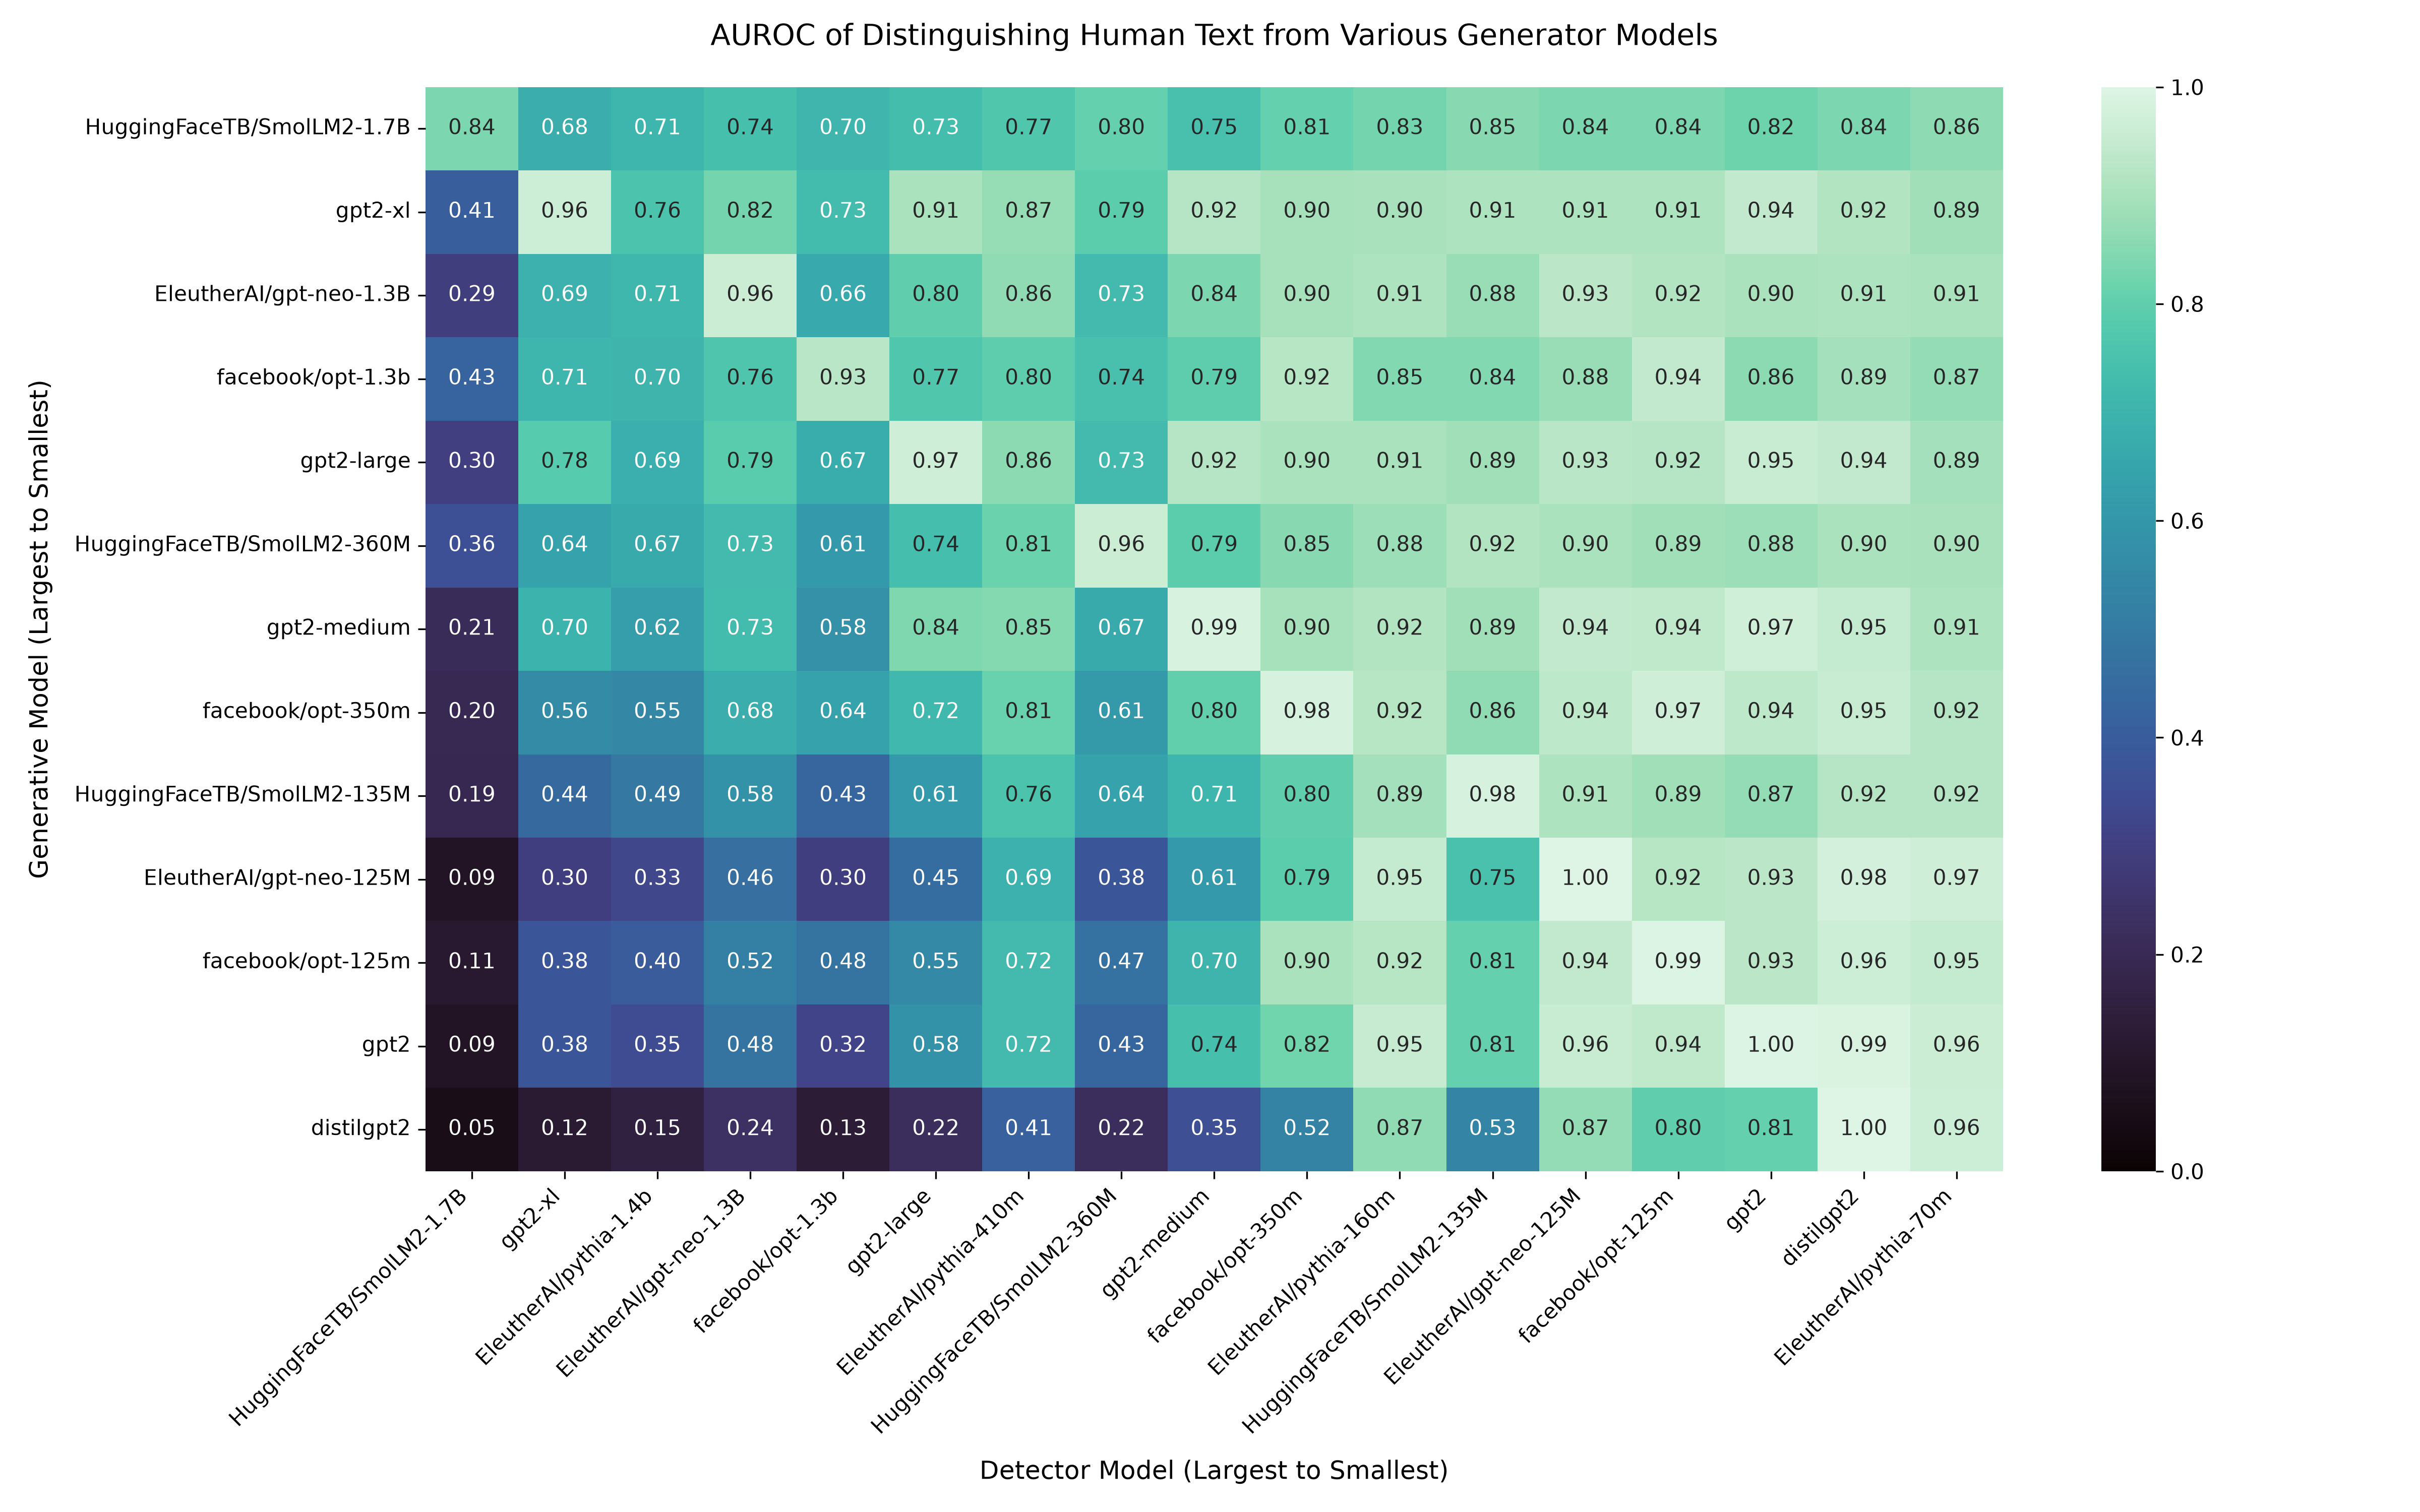
\includegraphics[width=\textwidth]{figures/Experiment1/auroc_heatmap.png}
\caption{AUROC scores for distinguishing human text from various generator models. Rows represent generative models and columns represent detector models, both sorted from largest to smallest parameter count, and lighter cells indicate higher performance. Detection efficacy is inversely related to detector size: the smallest detectors (right) exceed 0.90 against most generators whilst the largest (left) fall to or below chance.}
\label{fig:exp1_auroc}
\end{figure}
\begin{figure}[H]
\centering
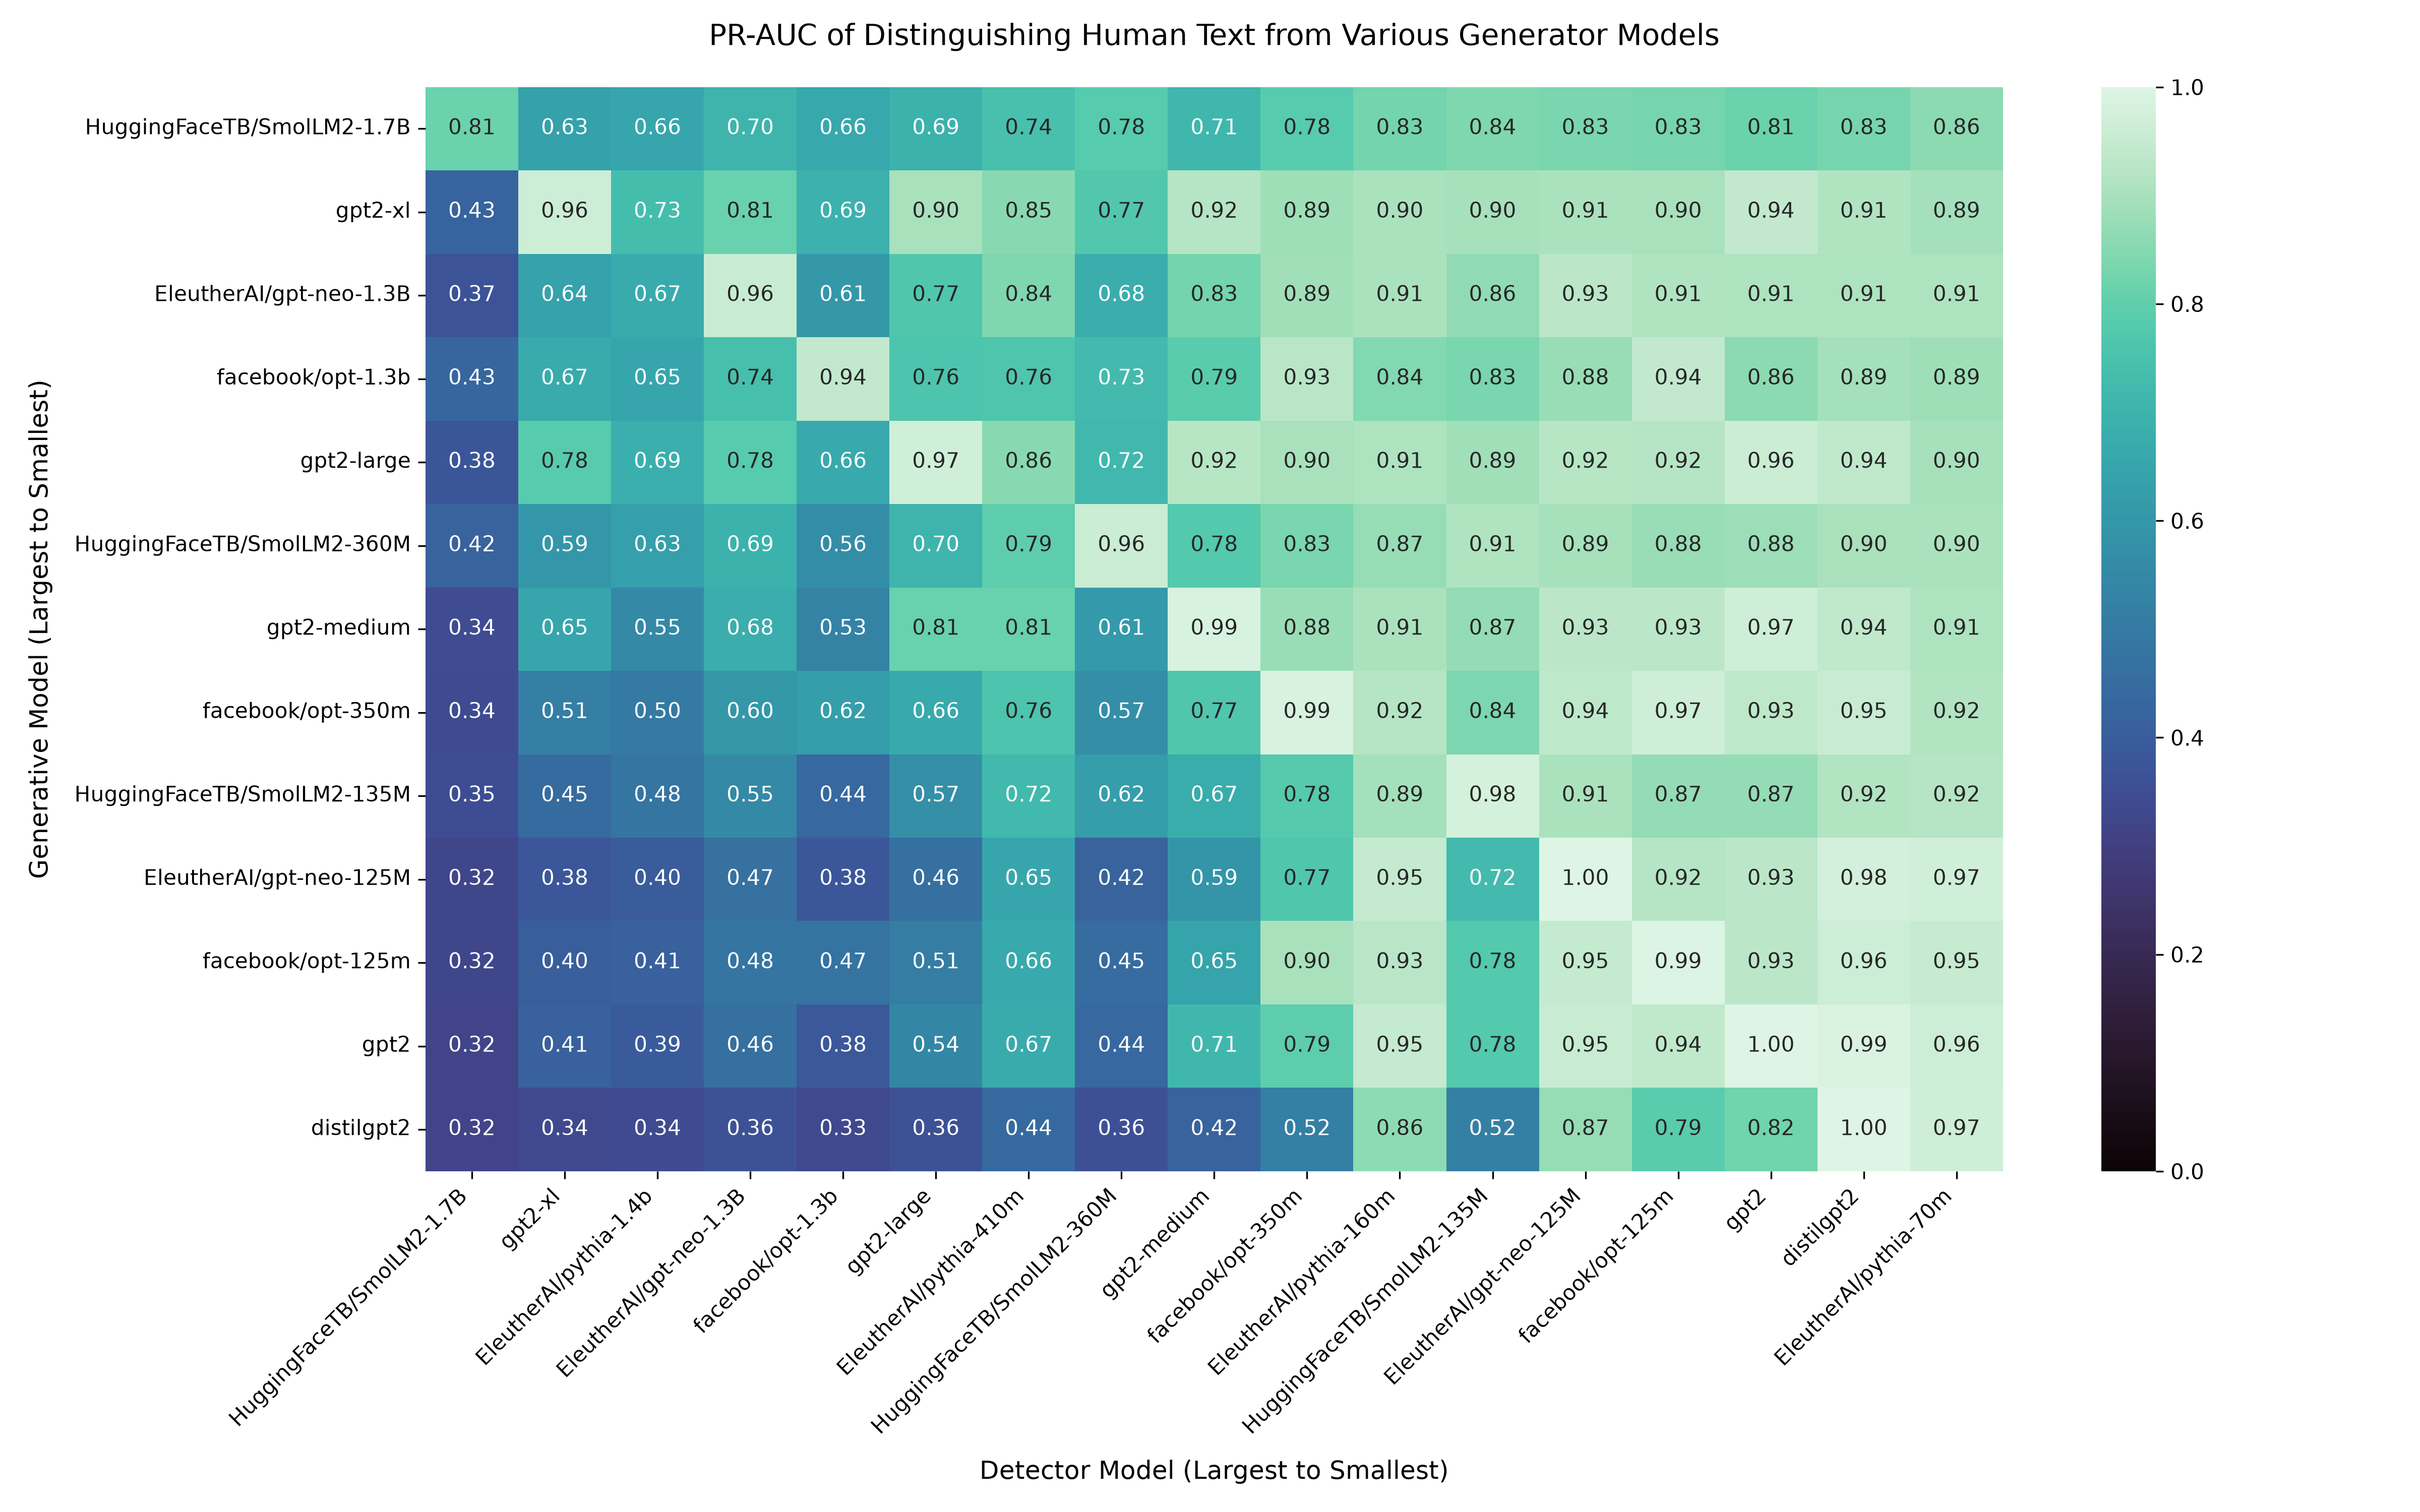
\includegraphics[width=\textwidth]{figures/Experiment1/prauc_heatmap.png}
\caption{PR-AUC scores for distinguishing human text from various generator models, with the same layout as Figure \ref{fig:exp1_auroc}. The gradient is identical, confirming that smaller detectors maintain high precision and recall whilst the largest detectors collapse.}
\label{fig:exp1_prauc}
\end{figure}
As illustrated in Figure \ref{fig:exp1_auroc}, the largest detectors, such as SmolLM2-1.7B and GPT-2 XL, perform poorly across almost all generators. The SmolLM2-1.7B detector scores between 0.05 and 0.43 AUROC, at or below random chance for most generators, and the GPT-2 XL detector fails on generators such as GPT-2 Medium (0.21 AUROC) and OPT-350M (0.20 AUROC). The smallest detectors, by contrast, are the strongest cross-detectors. Pythia-70M exceeds 0.90 AUROC for the majority of generators, including 0.86 against the much larger SmolLM2-1.7B generator, and DistilGPT-2 reaches 1.00 and 0.99 against GPT-2 and OPT-125M. The PR-AUC results in Figure \ref{fig:exp1_prauc} corroborate the AUROC picture, with smaller detectors maintaining high precision and recall whilst the largest detectors collapse.
The aggregate trend is confirmed in Figure \ref{fig:exp1_scale_trend}, which averages performance over the 13 generators and plots it against detector parameter count on a logarithmic axis. Mean AUROC declines monotonically from roughly 0.92 at 70 million parameters to around 0.27 at 1.7 billion, falling below the chance level at the largest scale, and mean PR-AUC follows the same trajectory from roughly 0.93 to 0.40. The decline is therefore an aggregate property of the matrix rather than an artefact of a few generator-detector pairs. The local dips, for example around 350 million parameters, reflect architectural family rather than scale, because the OPT and GPT-2 Medium detectors sit below the Pythia and SmolLM2 detectors of comparable size.
\begin{figure}[H]
\centering
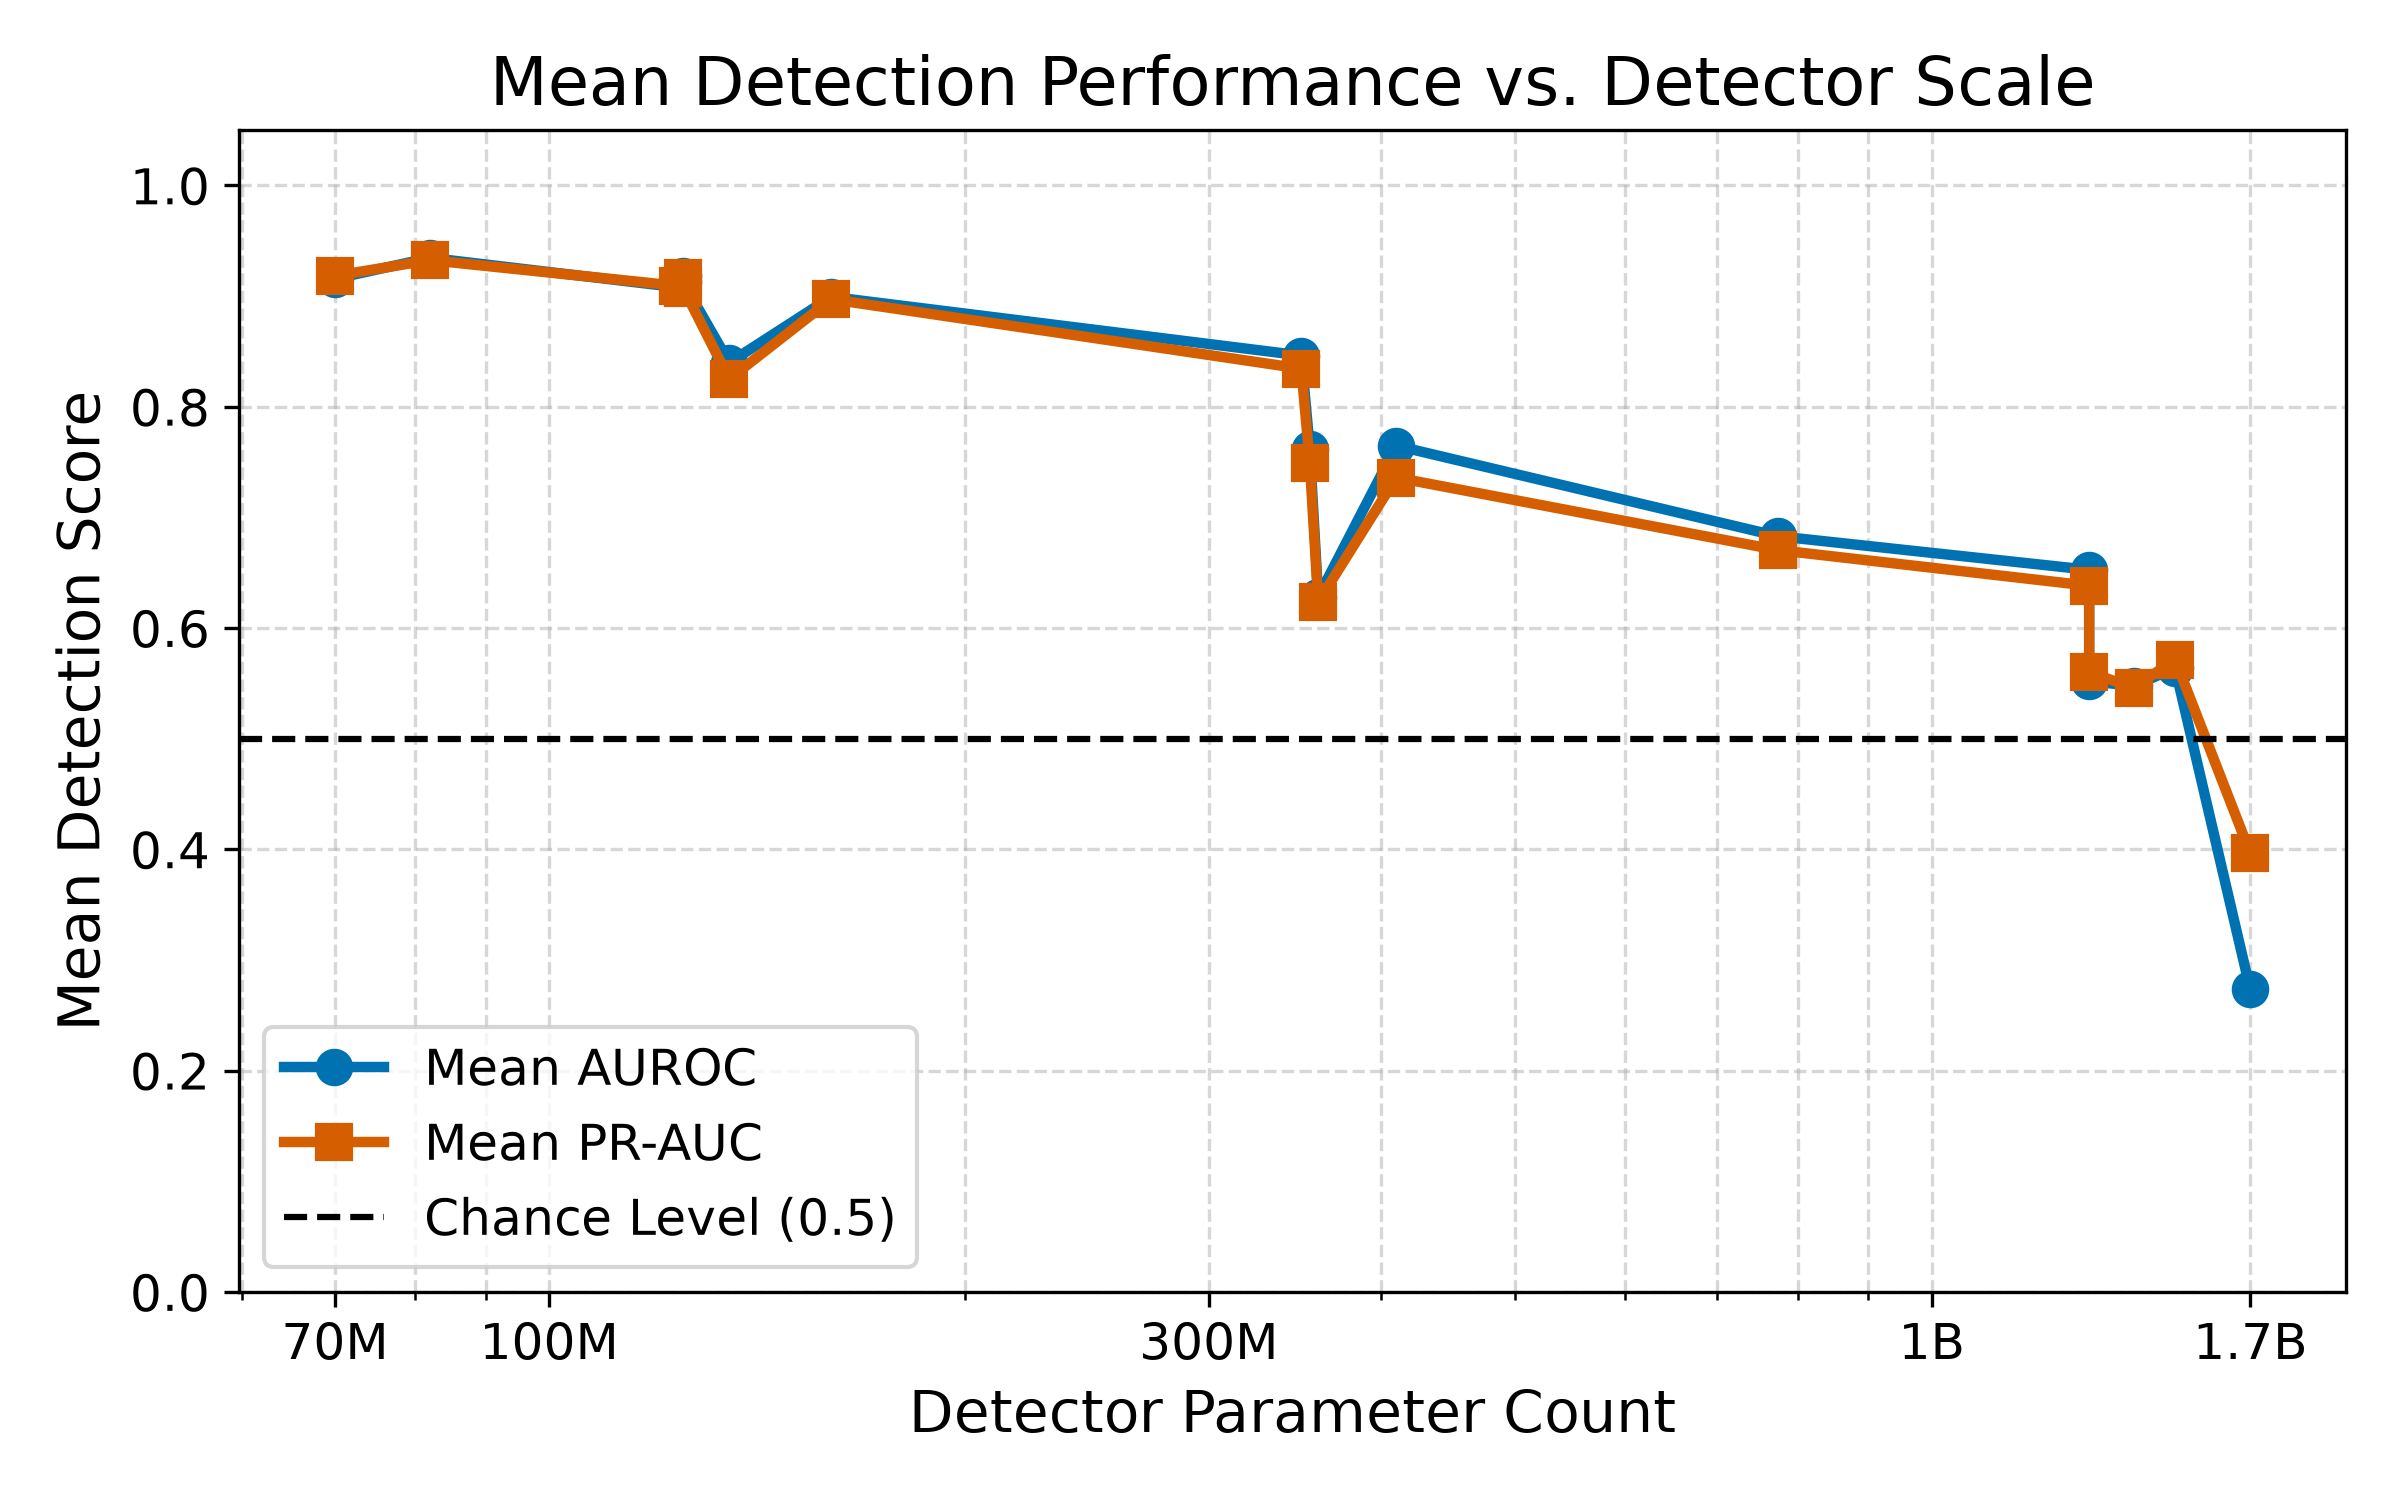
\includegraphics[width=0.75\textwidth]{figures/Experiment1/scale_trend.png}
\caption{Mean detection performance as a function of detector parameter count, averaged across the 13 generators. Both AUROC and PR-AUC decline monotonically as detector size increases and fall to or below the chance level (dashed line) at 1.7 billion parameters, confirming that the inverse relationship is an aggregate property of the matrix.}
\label{fig:exp1_scale_trend}
\end{figure}
Figure \ref{fig:exp1_family_split} separates within-family from cross-family detection for both metrics, to test whether the inverse relationship is driven by self-detection. A generator-detector pair is within-family when both belong to the same architectural family, for example a GPT-2 detector scoring GPT-2 text, and cross-family otherwise. Within-family performance exceeds cross-family performance at every scale, confirming that a detector recognises its own sampling distribution. However, all four curves decline monotonically with scale and collapse together at 1.7 billion parameters, where within-family AUROC falls to roughly 0.46 and cross-family AUROC to roughly 0.21, and the PR-AUC panels show the same collapse. The within-family advantage therefore attenuates but does not reverse the effect of scale, and the inverse relationship is not an artefact of self-detection.
\begin{figure}[H]
\centering
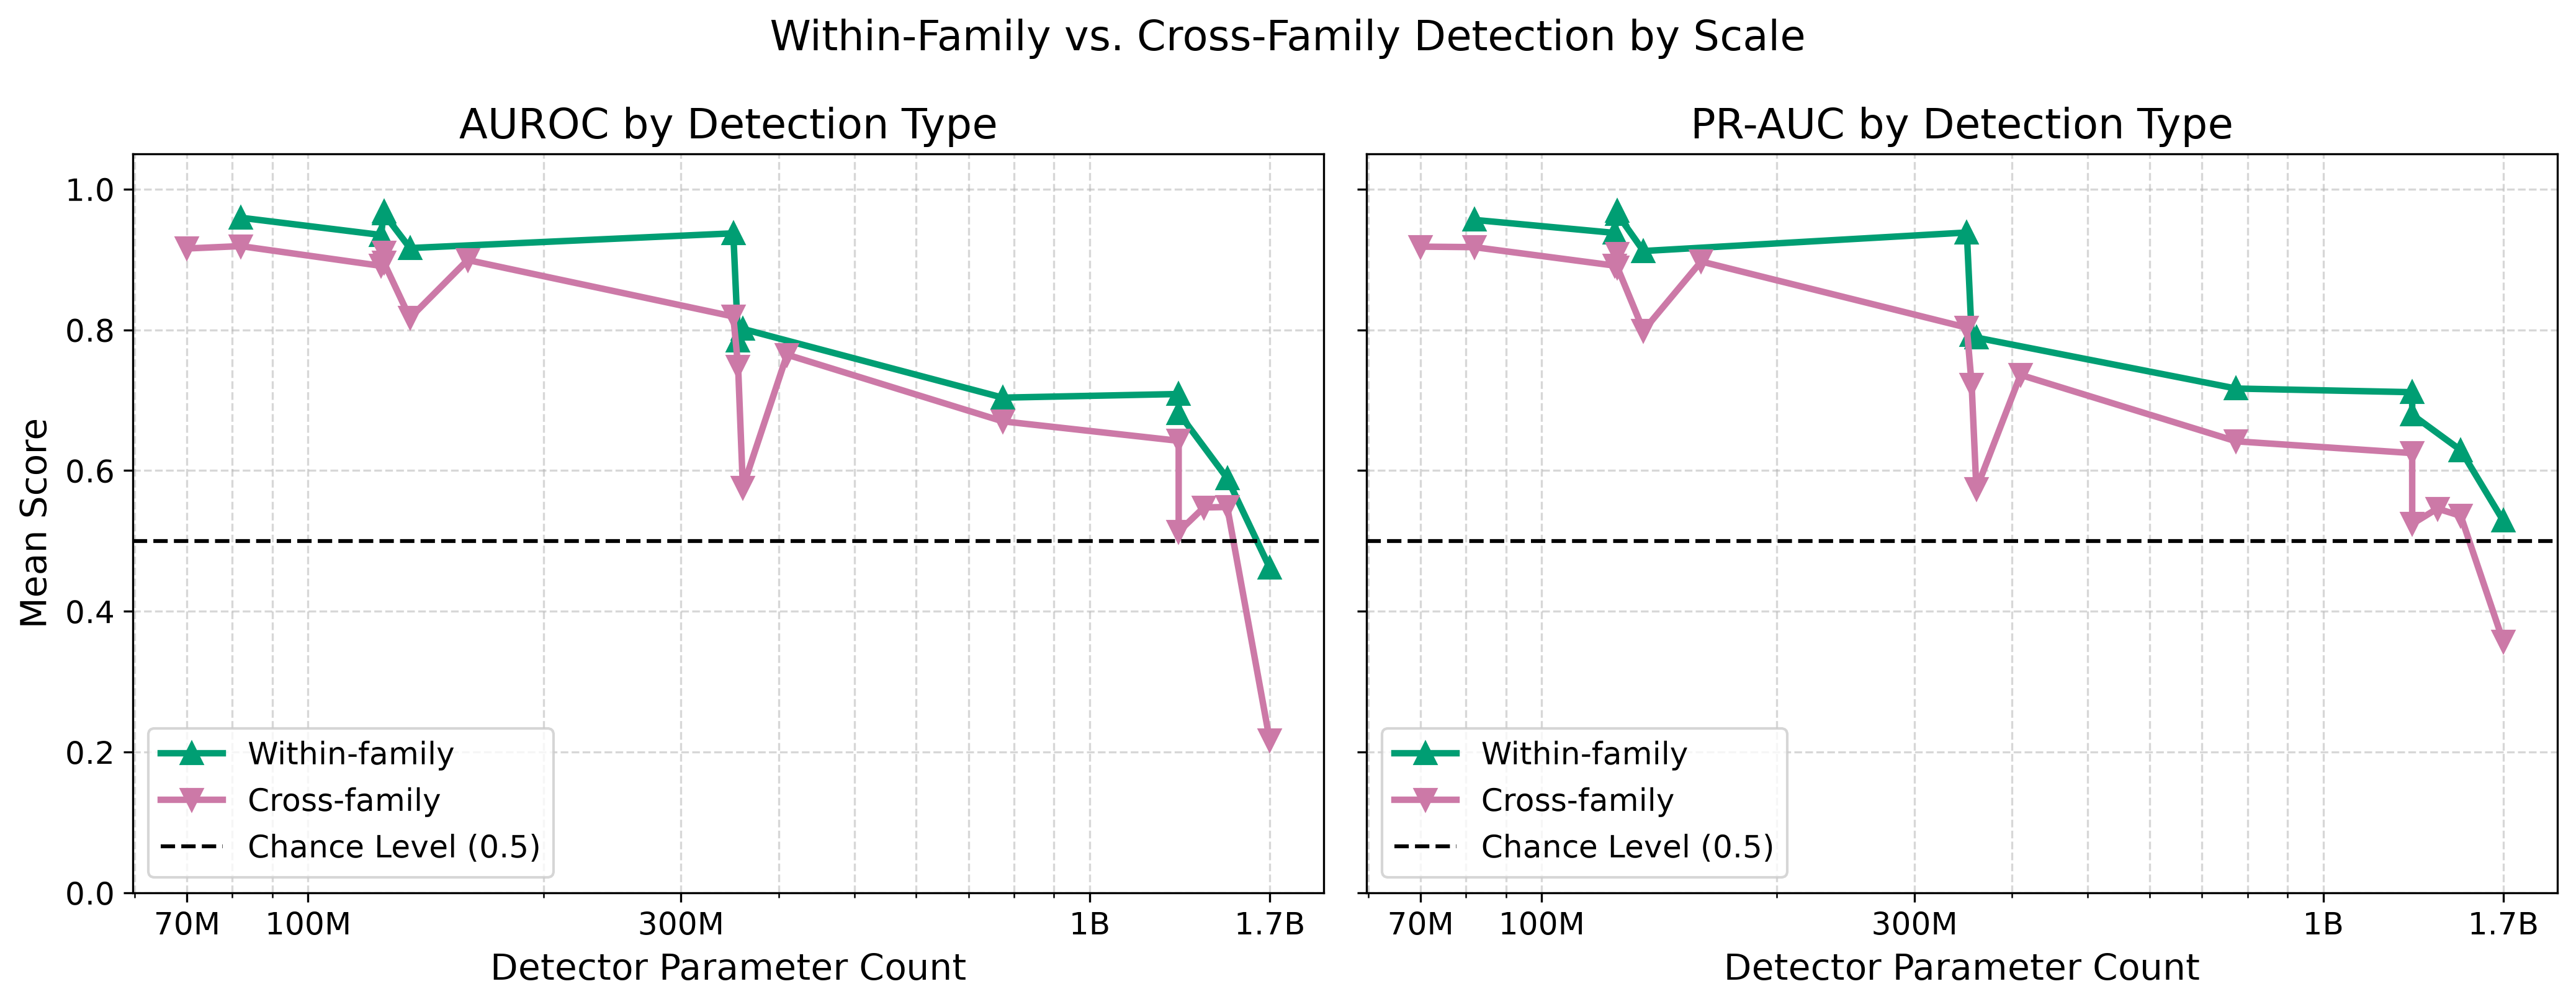
\includegraphics[width=0.75\textwidth]{figures/Experiment1/scale_trend_family_split.png}
\caption{Within-family and cross-family mean AUROC (left) and PR-AUC (right) by detector scale. Within-family performance exceeds cross-family performance at every scale for both metrics, but all four curves decline monotonically and collapse together at 1.7 billion parameters, showing that the inverse relationship is not driven by self-detection. Pythia detectors appear only in the cross-family curves because Pythia models were not used as generators.}
\label{fig:exp1_family_split}
\end{figure}

\section{Mechanistic and Distributional Analysis}
\label{sec:exp1_analysis}
The inverse relationship is best understood through the geometry of the likelihood surface and the calibration behaviour of large models. Larger language models are known to become better calibrated and more confident as they scale \citep{guo2017calibration, kadavath2022language}. Calibration, in this setting, is the tendency of a model's stated probabilities to be reliable and well spread; a more confident model assigns high probability to a broad set of plausible continuations, which smooths the local likelihood surface and reduces the local gradient that the curvature metric exploits. Larger models also have greater capacity to absorb distributional variation, which flattens the local minima that the curvature metric relies upon \citep{belkin2019reconciling}.
Smaller models, by contrast, are less calibrated and assign sharper, more differentiated probabilities. A perturbation to machine text therefore produces a large and consistent drop in log probability, whilst human text, which occupies a broader region of the surface, absorbs the same disruption with a smaller relative drop. The divergence between the two classes is therefore largest for the smallest detectors, producing the strong separation seen in the heatmaps. This account also explains the self-family pattern in Figure \ref{fig:exp1_family_split}: a detector detects its own family well at small scale because it recognises its own sampling distribution, but this recognition fades as the surface smooths with scale, which is why the within-family curves collapse alongside the cross-family curves for both metrics.

\section{Discussion and Summary}
\label{sec:exp1_summary}
This experiment establishes a foundational finding for the comparative analysis: smaller detector models consistently outperform their larger counterparts in curvature-based text detection. The heatmaps demonstrate that massive parameter counts are not only unnecessary for effective detection but are actively detrimental to cross-architecture generalisation. The superior performance of models like Pythia-70M and DistilGPT-2 validates the hypothesis that sharper likelihood surfaces, characteristic of Small Language Models, provide the necessary sensitivity to distinguish the negative curvature signatures of machine-generated text.
Scale was isolated by holding the perturbation stage fixed at the semantic control and restricting the evaluation to the zero-shot setting on a single corpus. The interaction between detector size and perturbation strategy is examined for a subset of detectors in Chapters \ref{chap:exp3} and \ref{chap:exp4}, whilst the zero-shot and single-corpus constraints remain global scope boundaries of this dissertation, which are revisited as limitations in the concluding chapter.
The optimal parameter scale is crucial, but the state of a model's weights at a given scale is equally important. The sharpness of a likelihood surface is not static; it evolves continuously as a neural network minimises its loss function. Large models often suffer from overconfidence as they converge, but it remains unclear whether smaller models experience a similar degradation in their likelihood surface geometry as they reach full convergence. Because smaller models possess inherently better detection characteristics, the next chapter moves from parameter scale to training dynamics. Chapter \ref{chap:exp2} evaluates how the evolution of detector weights over time affects the sharpness of the likelihood surface, specifically testing whether partially trained checkpoints offer a superior decision boundary compared to fully converged models.

\chapter{Experiment 2: Training Checkpoint Dynamics}
\label{chap:exp2}
This chapter asks a second counter-intuitive question: does a better-trained detector make a better detector? The standard practice in machine learning is to train to convergence, that is, until the training loss stops falling, yet the results show the opposite for curvature-based detection. Across a 13-generator by 18-detector-checkpoint matrix, detection efficacy, the ability to separate human from machine text, is inversely related to training duration, and partially trained checkpoints emerge as the strongest cross-detectors, detectors that work well on generators they have never seen. The aggregate trend adds a sharper point: at the earliest checkpoint all three detector scales perform almost identically, and the harm of scale only appears as training proceeds. This chapter establishes these facts, quantifies them, and offers a mechanistic account in terms of overfitting, in which the model memorises its training data rather than learning general patterns, and the resulting smoothing of the likelihood surface.

\section{Experimental Setup}
\label{sec:exp2_setup}
The experiment evaluates how the evolution of detector weights over time affects detection efficacy, holding the generator suite and the perturbation stage fixed. The generators remain identical to Chapter \ref{chap:exp1}, spanning 13 architectures from 82 million to 1.7 billion parameters.
The detectors are restricted to the Pythia family at three scales, Pythia-1.4B, Pythia-410M and Pythia-70M, because the Pythia suite releases 154 checkpoints per model trained on identical data, giving unprecedented visibility into learning dynamics \citep{biderman2023pythia}. A checkpoint is a saved copy of the model's weights at a given training step, where a training step is one batch of weight updates. From this suite, six checkpoints are extracted: 1,000, 5,000, 10,000, 50,000, 100,000 and 143,000 steps, giving a high-resolution view of early training alongside the mid-training and convergence stages. This yields a matrix of 13 generators against 18 detector configurations, evaluated on 250 human-written and 250 machine-generated samples per generator with the semantic control of Chapter \ref{chap:exp3}, the T5-large mask-filler. Performance is reported as AUROC, the probability that a randomly drawn machine document outscores a randomly drawn human document, and PR-AUC; on this balanced dataset a score of 0.5 is no better than a coin flip.

\section{Quantitative Results}
\label{sec:exp2_results}
The full matrix is shown in Figure \ref{fig:exp2_auroc} (AUROC) and Figure \ref{fig:exp2_prauc} (PR-AUC). The dominant pattern is an inverse relationship between training duration and detection efficacy.
\begin{figure}[H]
\centering
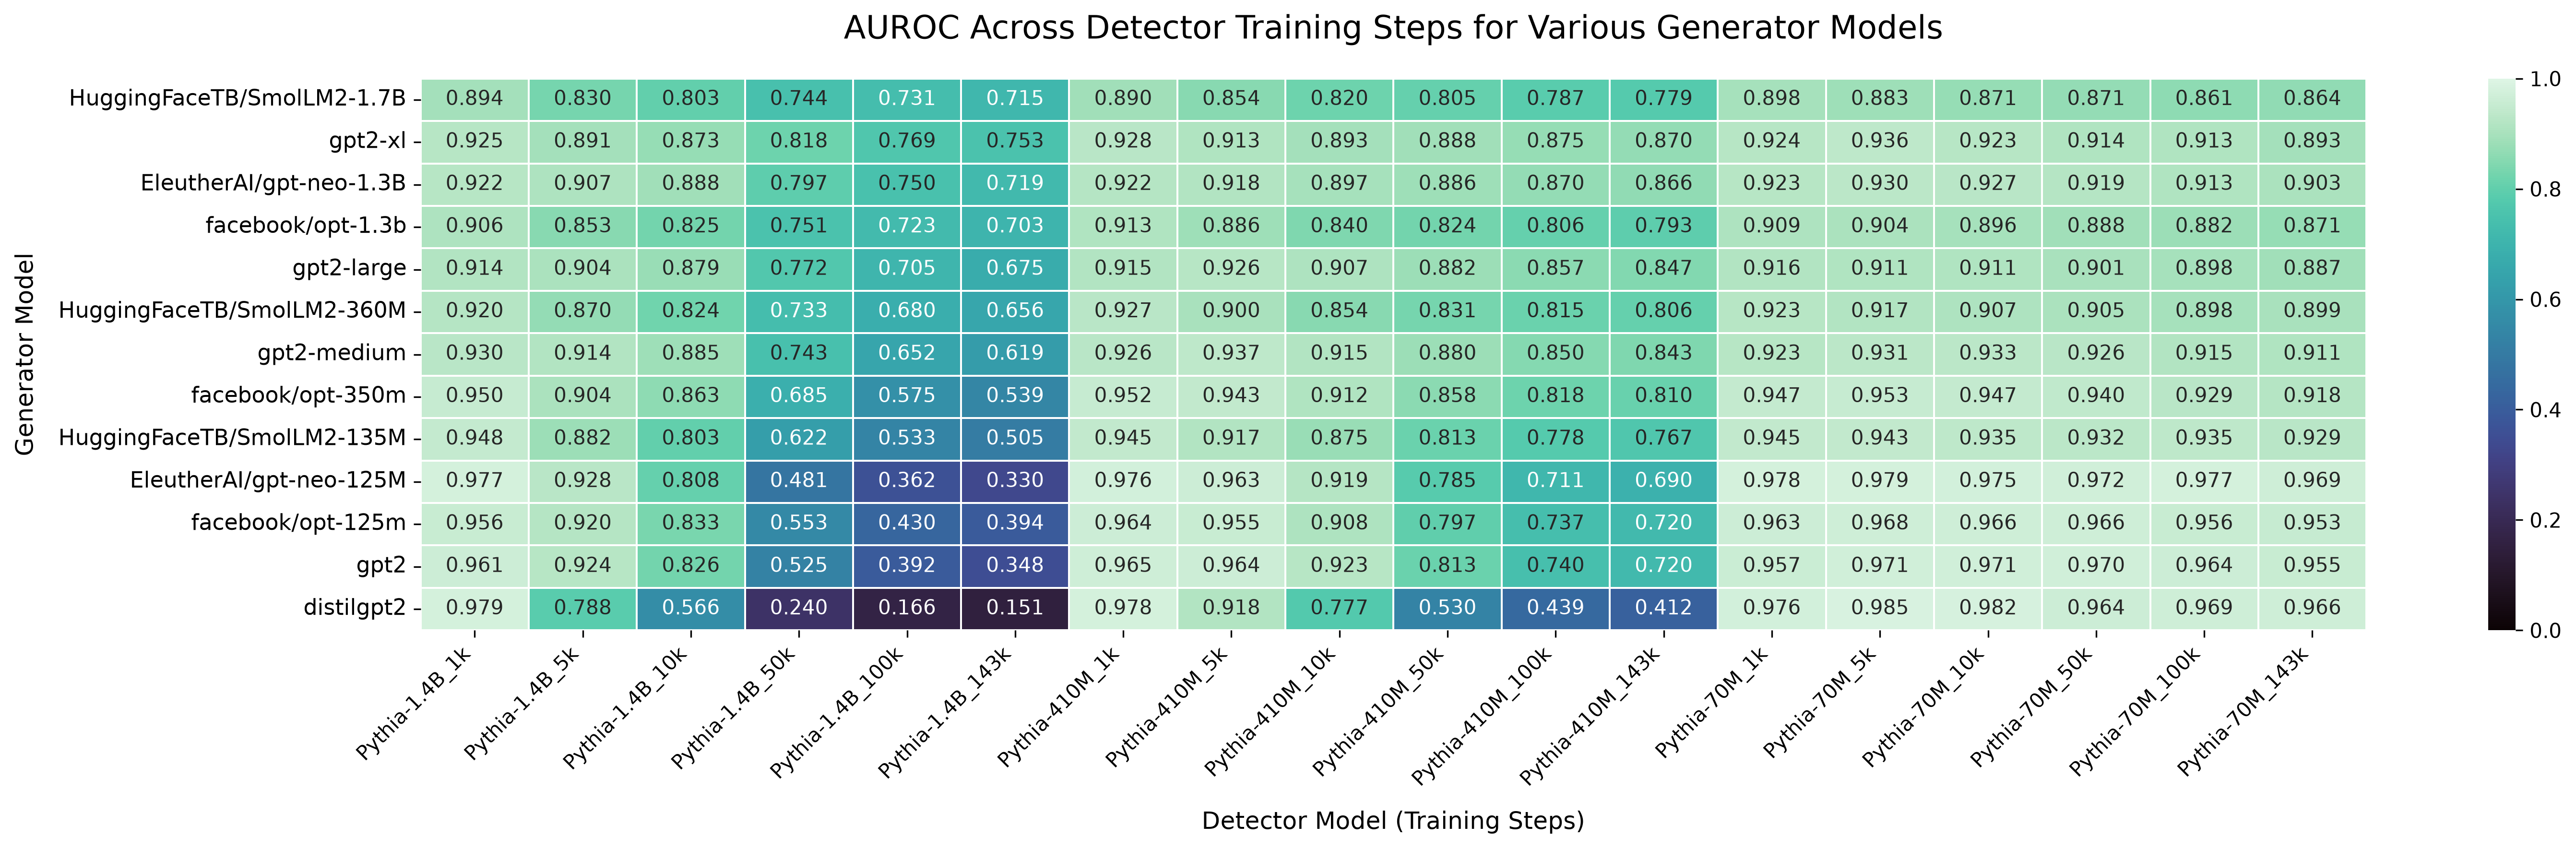
\includegraphics[width=\textwidth]{figures/Experiment2/auroc_heatmap.png}
\caption{AUROC scores across detector training steps for various generator models. Rows represent generative models and columns represent detector checkpoints, sorted by model size and training progression, and lighter cells indicate higher performance. Detection efficacy is inversely related to training duration: early checkpoints exceed 0.90 against most generators whilst fully converged checkpoints fall to or below chance, most severely for Pythia-1.4B.}
\label{fig:exp2_auroc}
\end{figure}
\begin{figure}[H]
\centering
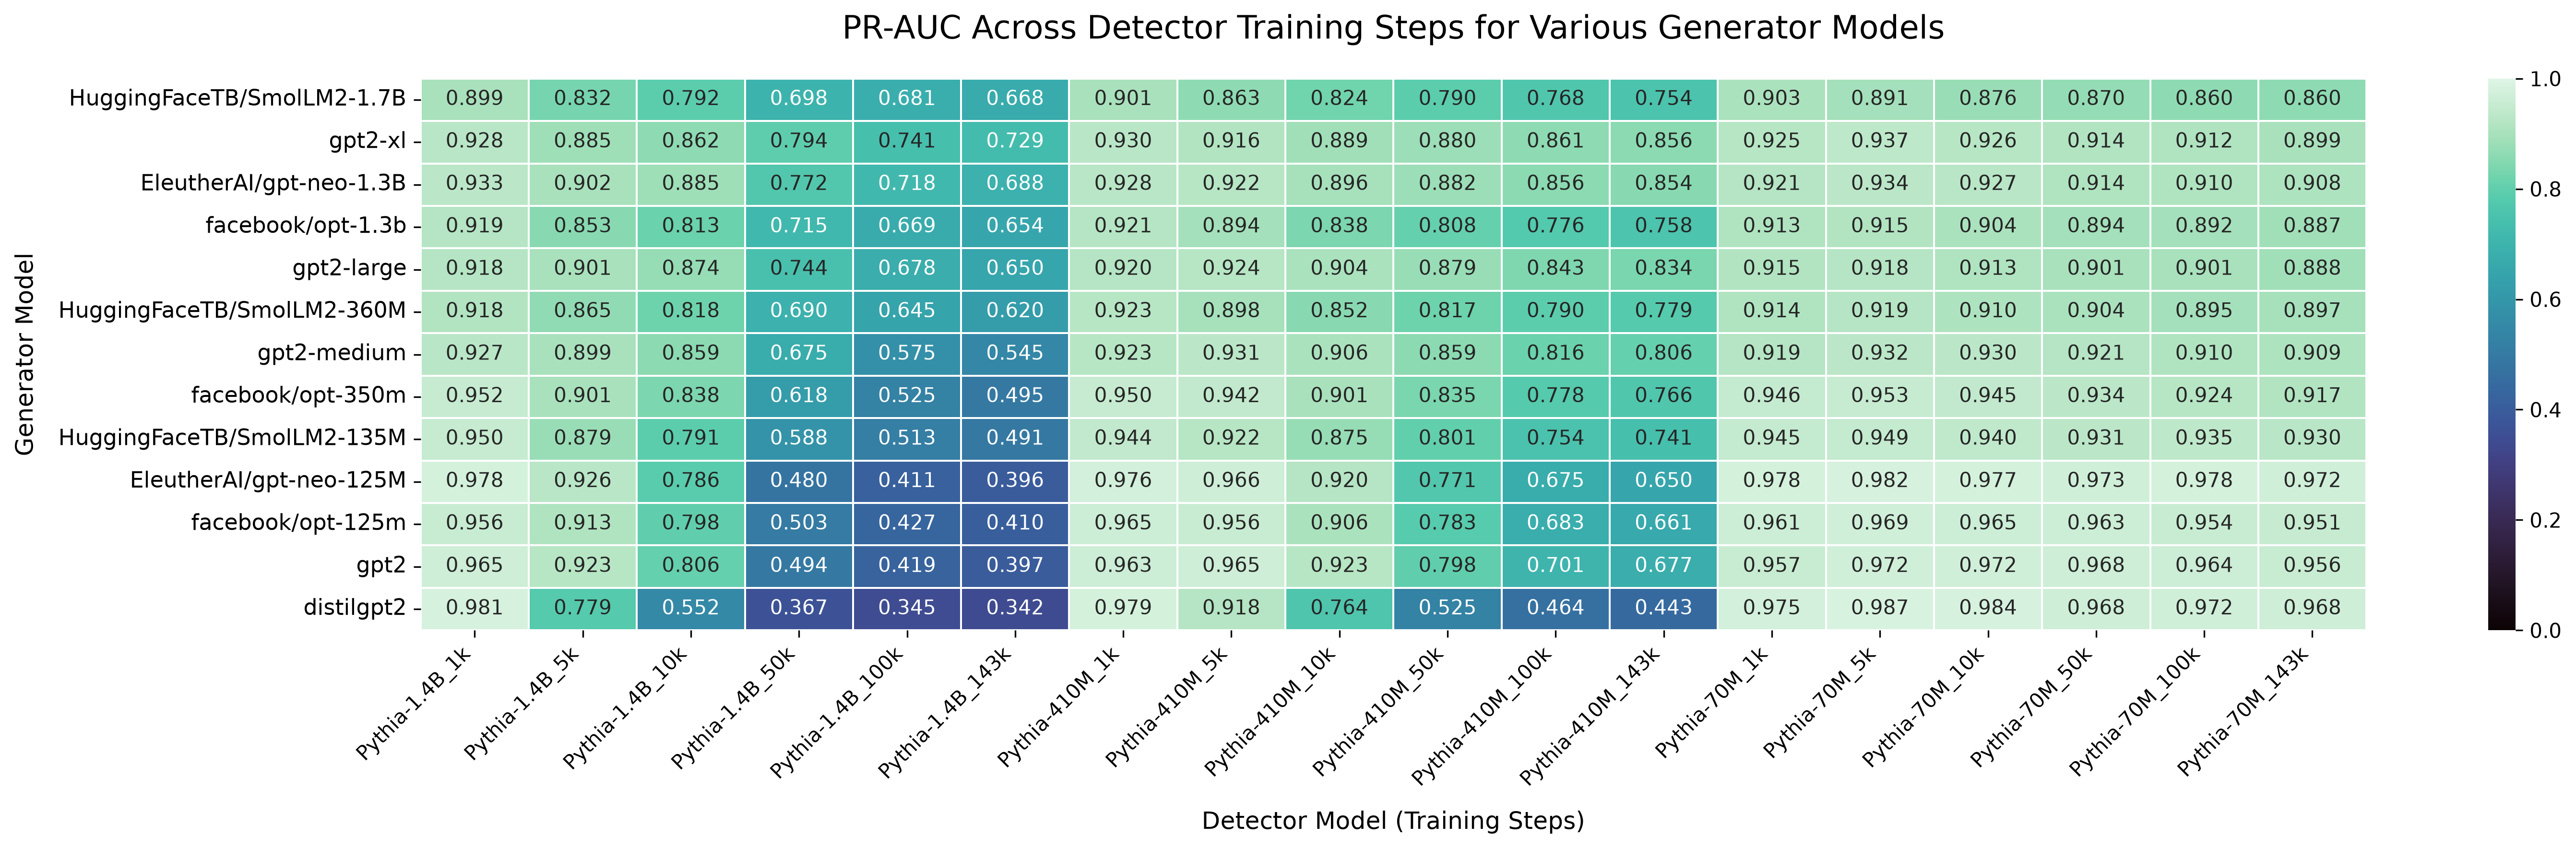
\includegraphics[width=\textwidth]{figures/Experiment2/prauc_heatmap.png}
\caption{PR-AUC scores across detector training steps for various generator models, with the same layout as Figure \ref{fig:exp2_auroc}. The gradient is identical and more severe, confirming that full convergence collapses precision and recall, especially for the largest detector.}
\label{fig:exp2_prauc}
\end{figure}
As illustrated in Figure \ref{fig:exp2_auroc}, the earliest checkpoints (1k, 5k and 10k steps) consistently achieve the highest performance across all detector scales. The Pythia-70M detector at 1k steps exceeds 0.95 AUROC for the majority of generators, including 0.898 against the larger SmolLM2-1.7B generator, and the Pythia-410M detector at 1k steps scores between 0.890 and 0.978 across generators.
The fully converged checkpoints (50k, 100k and 143k steps) show severe degradation, most pronounced in the largest detector. At 143k steps, Pythia-1.4B falls to 0.151 AUROC on DistilGPT-2 and 0.330 on GPT-Neo-125M, at or below chance, whilst the smaller Pythia-70M degrades only mildly, dropping from 0.976 to 0.966 on GPT-2. The PR-AUC results in Figure \ref{fig:exp2_prauc} corroborate this with greater severity, with Pythia-1.4B at 143k steps reaching 0.342 and 0.396 PR-AUC on the same generators.
The aggregate trend is confirmed in Figure \ref{fig:exp2_checkpoint_trend}, which averages performance over the 13 generators and plots it against training step for each detector scale. Two features stand out. First, the three scales start almost together: at 1k steps all three detectors attain roughly 0.94 mean AUROC and 0.94 mean PR-AUC, so at the earliest checkpoint parameter count barely matters. Second, the curves diverge monotonically as training proceeds: by 143k steps Pythia-1.4B falls to about 0.55 mean AUROC, within a few points of the chance level, Pythia-410M to about 0.77, and Pythia-70M only to about 0.92. The magnitude of degradation therefore grows with parameter count, and the optimal window lies between 1k and 10k steps. The PR-AUC panel shows the same pattern with slightly greater severity, with Pythia-1.4B ending near 0.54.
\begin{figure}[H]
\centering
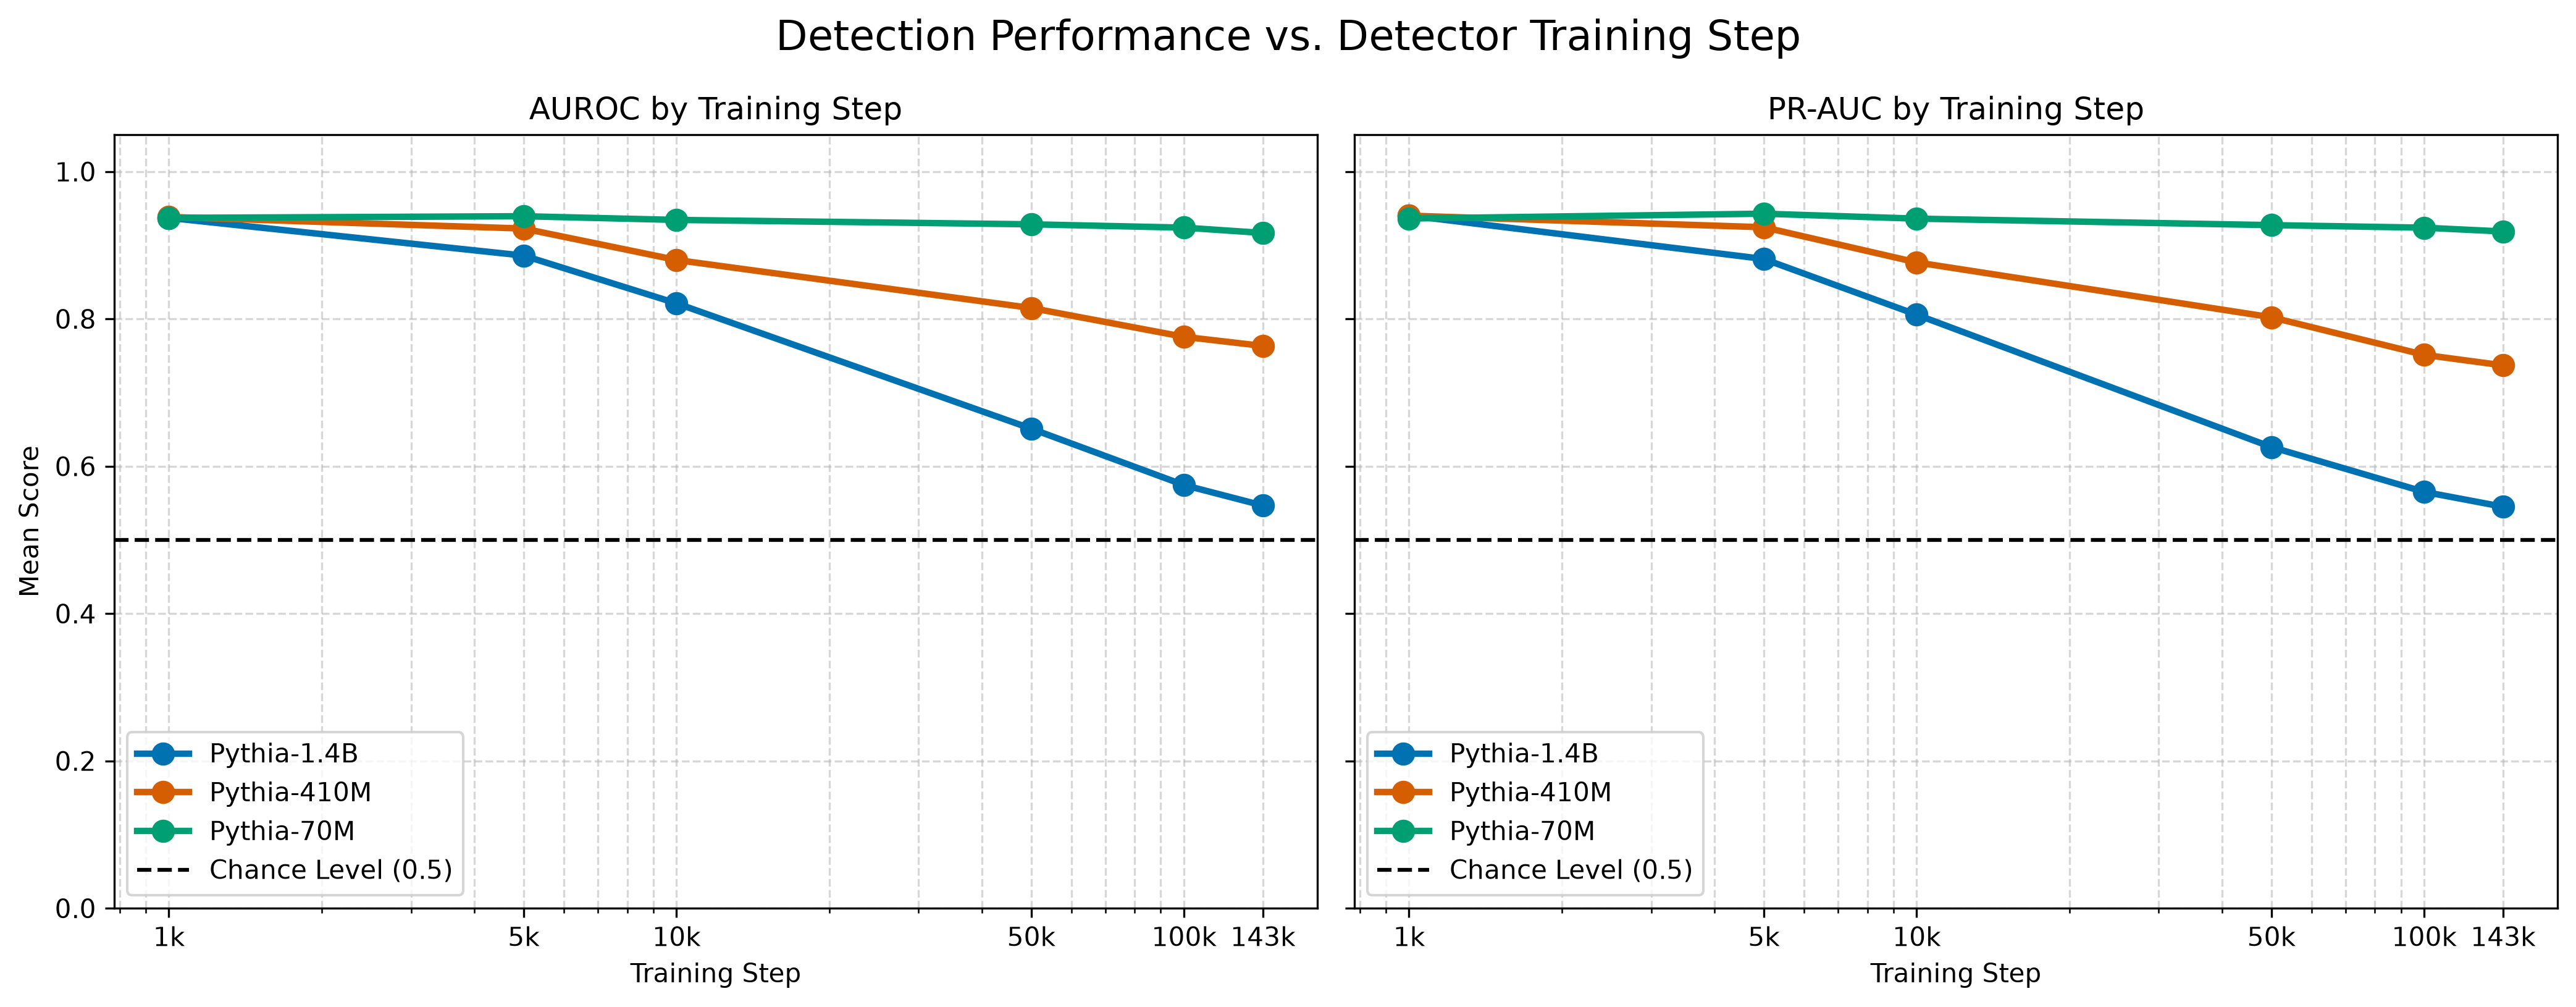
\includegraphics[width=\textwidth]{figures/Experiment2/checkpoint_trend.png}
\caption{Mean detection performance as a function of detector training step, averaged across the 13 generators. All three scales start near 0.94 at 1k steps, but the degradation grows with parameter count: by 143k steps Pythia-1.4B falls to about 0.55 (near the dashed chance line), Pythia-410M to about 0.77, and Pythia-70M only to about 0.92, showing that overfitting, not scale alone, drives the decline.}
\label{fig:exp2_checkpoint_trend}
\end{figure}

\section{Mechanistic and Distributional Analysis}
\label{sec:exp2_analysis}
The inverse relationship is best understood as an overfitting phenomenon. During early training, the detector possesses broad and less specialised probability distributions: it has learned enough linguistic structure to assign meaningful probabilities, but has not yet memorised the statistical artefacts of its training corpus, so the likelihood surface retains the sensitivity needed to separate human from machine text. As training progresses, the model overfits to its training distribution and the likelihood surface becomes increasingly conservative and smooth, mirroring the behaviour of large pretrained models in Chapter \ref{chap:exp1}. Perturbations, the small edits of Equation~\ref{eq:curvature}, then produce minimal changes in log probability for both classes, and the curvature score collapses towards zero.
This account is consistent with the broader literature on training dynamics, in which longer training can hurt out-of-distribution generalisation \citep{nakkiran2021deep}, and with the sharp-minima literature, in which the geometry of the minima a network settles into governs its generalisation \citep{keskar2016large}. The interaction with scale follows directly: larger models have greater capacity to memorise their training data and therefore overfit more severely, whilst the limited capacity of Pythia-70M acts as an implicit regulariser, a built-in brake on memorisation, that preserves sharper probability gradients even at full convergence.
The convergence of the three curves at 1k steps reframes the scale effect of Chapter \ref{chap:exp1}. In that experiment every detector was evaluated fully converged, so parameter count and overfitting were confounded: the large detectors were harmful partly because they were the most overfit. A Pythia-1.4B at 1k steps matches a Pythia-70M at any checkpoint, which shows that a large likelihood surface is not irredeemably smooth; it is the converged large surface that is. Detection efficacy is therefore not merely a function of scale, but of the interaction between scale and training state, and the strongest detector is a small model at an early checkpoint.

\section{Discussion and Summary}
\label{sec:exp2_summary}
This experiment establishes a second foundational result: partially trained detectors consistently outperform fully converged checkpoints, with an optimal window between 1,000 and 10,000 steps. The practical message is direct: training a curvature detector to full convergence, the standard practice, is actively detrimental, and practitioners should instead halt training early or use partially trained checkpoints, a recommendation with clear precedent in the early-stopping literature \citep{prechelt2002early}. Early stopping means halting training before convergence on purpose, which is exactly the move this chapter recommends.
Combined with Chapter \ref{chap:exp1}, the finding identifies the strongest detector configuration as a small model at an early checkpoint, which sharpens the central practical claim of this dissertation. Two scope boundaries qualify this chapter. The checkpoint analysis is restricted to the Pythia family, and the perturbation stage was held fixed at the semantic control, so the interaction between training state and perturbation quality is not characterised here; that interaction is examined for a subset of detectors in Chapters \ref{chap:exp3} and \ref{chap:exp4}. Chapter \ref{chap:exp3} now shifts focus from the detector to the perturbation pipeline, evaluating how the capacity of the mask-filling model influences detection accuracy.

\chapter{Experiment 3: Semantic Perturbation Scale}
\label{chap:exp3}
This chapter asks a third question: how much of the detection budget must be spent on constructing the perturbation neighbourhood, the set of edited copies that the curvature score averages over? The curvature metric is only as reliable as those neighbours, and the canonical pipeline spends most of its compute on a large mask-filling model, the second model that rewrites the masked blanks. The results show that this spend is largely wasteful: performance rises monotonically with mask-filler capacity, the parameter count of the filling model, but with clear diminishing returns, and a small detector paired with a medium filler recovers nearly all of the available signal. This chapter quantifies that trade-off and explains why a weak filler destroys the signal of a large detector but not of a small one.

\section{Experimental Setup}
\label{sec:exp3_setup}
The third experiment isolates the capacity of the mask-filling model as the manipulated constituent. The generator is fixed to SmolLM2-1.7B \citep{allal2024smollm}, the model that wrote the machine text and the strongest generator examined in the preceding experiments, so that the quality of the synthetic text is held constant at a high level. The detector suite comprises the three Pythia checkpoints that span the relevant range of likelihood-surface sharpness in Chapter \ref{chap:exp2}, namely Pythia-1.4B, Pythia-410M and Pythia-70M \citep{biderman2023pythia}.
The perturbation stage follows the masking protocol of DetectGPT \citep{mitchell2023detectgpt}: 30\% of the tokens in each document are masked in spans of length two, that is, pairs of consecutive words are hidden, and 50 perturbed variants, edited copies, are drawn for every sample. Three mask-filling models from the T5 family, sequence-to-sequence models trained to rewrite masked spans \citep{raffel2020exploring}, are compared, namely T5-small, T5-large and T5-3B, with roughly 60 million, 770 million and 3 billion parameters respectively, spanning two orders of magnitude in capacity. This yields a three by three matrix of detector and mask-filler configurations, evaluated on 250 human-written and 250 machine-generated samples. Performance is reported as AUROC, the probability that a randomly drawn machine document outscores a randomly drawn human document, and PR-AUC; on this balanced dataset a score of 0.5 is no better than a coin flip.

\section{Quantitative Results}
\label{sec:exp3_results}
Figure \ref{fig:exp3_bars} reports the AUROC and PR-AUC attained by each detector under the three mask-filling models, and Figure \ref{fig:exp3_curves} shows the corresponding ROC and PR curves. Two consistent trends emerge.
\begin{figure}[H]
\centering
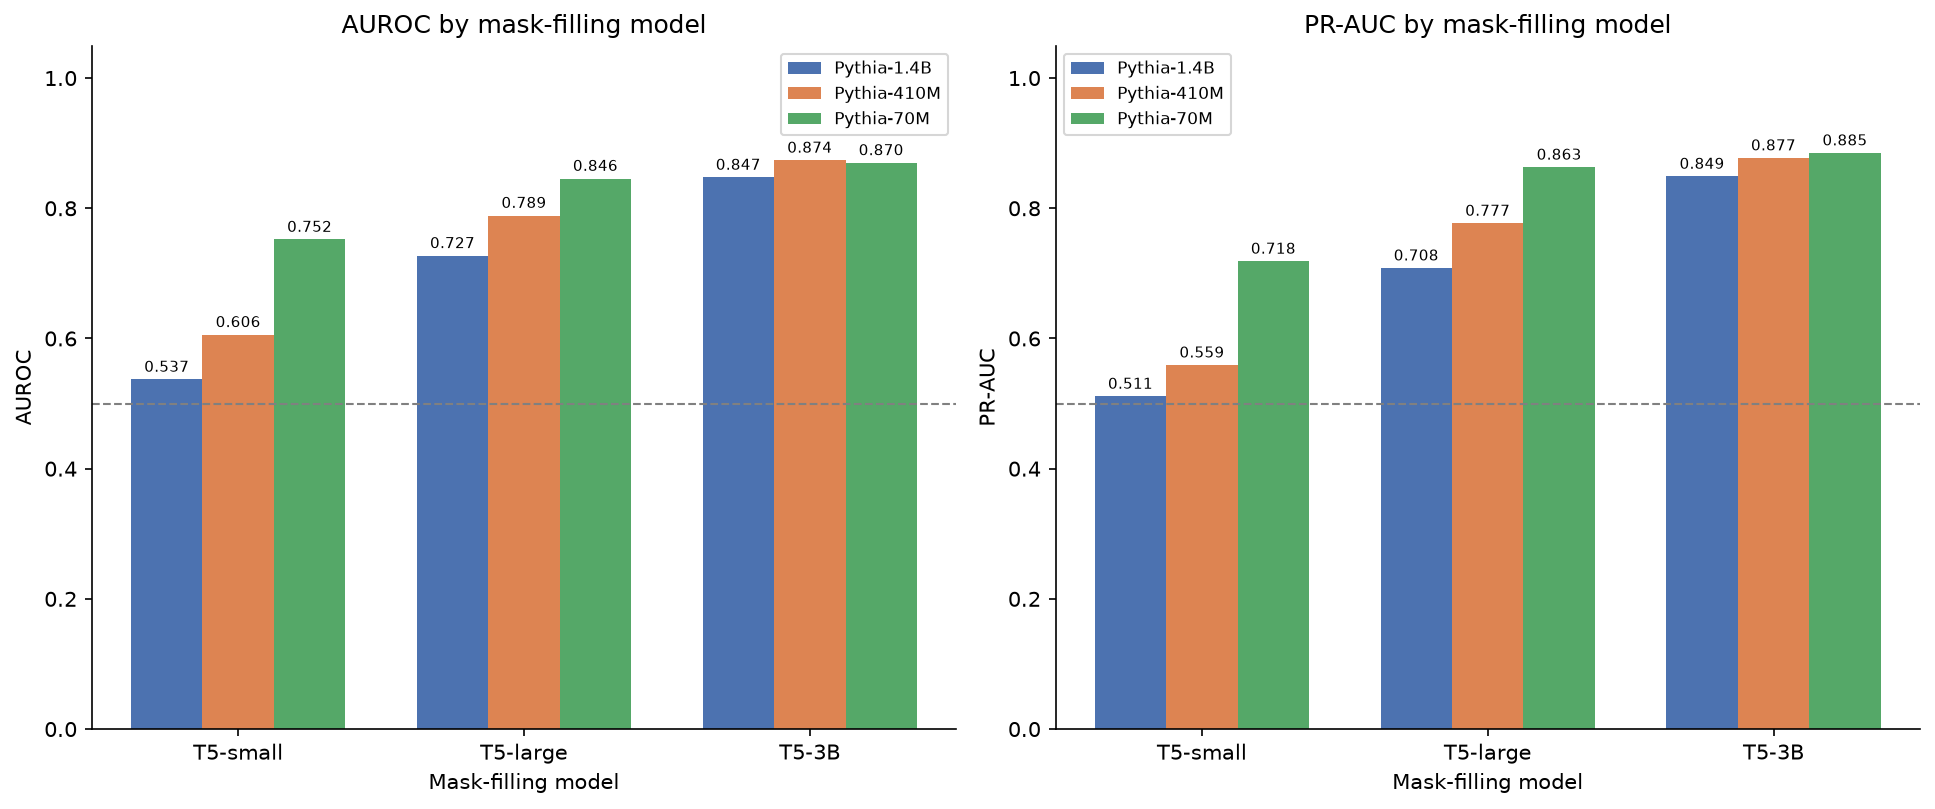
\includegraphics[width=\textwidth]{figures/Experiment3/perturbation_scale_bars.png}
\caption{Detection performance of the three Pythia detectors under the three T5 mask-filling models. Left: AUROC. Right: PR-AUC. Performance rises monotonically with filler capacity for every detector, but the gain from T5-large to T5-3B is small, and T5-small collapses the large detectors to near the dashed chance line.}
\label{fig:exp3_bars}
\end{figure}
\begin{figure}[H]
\centering
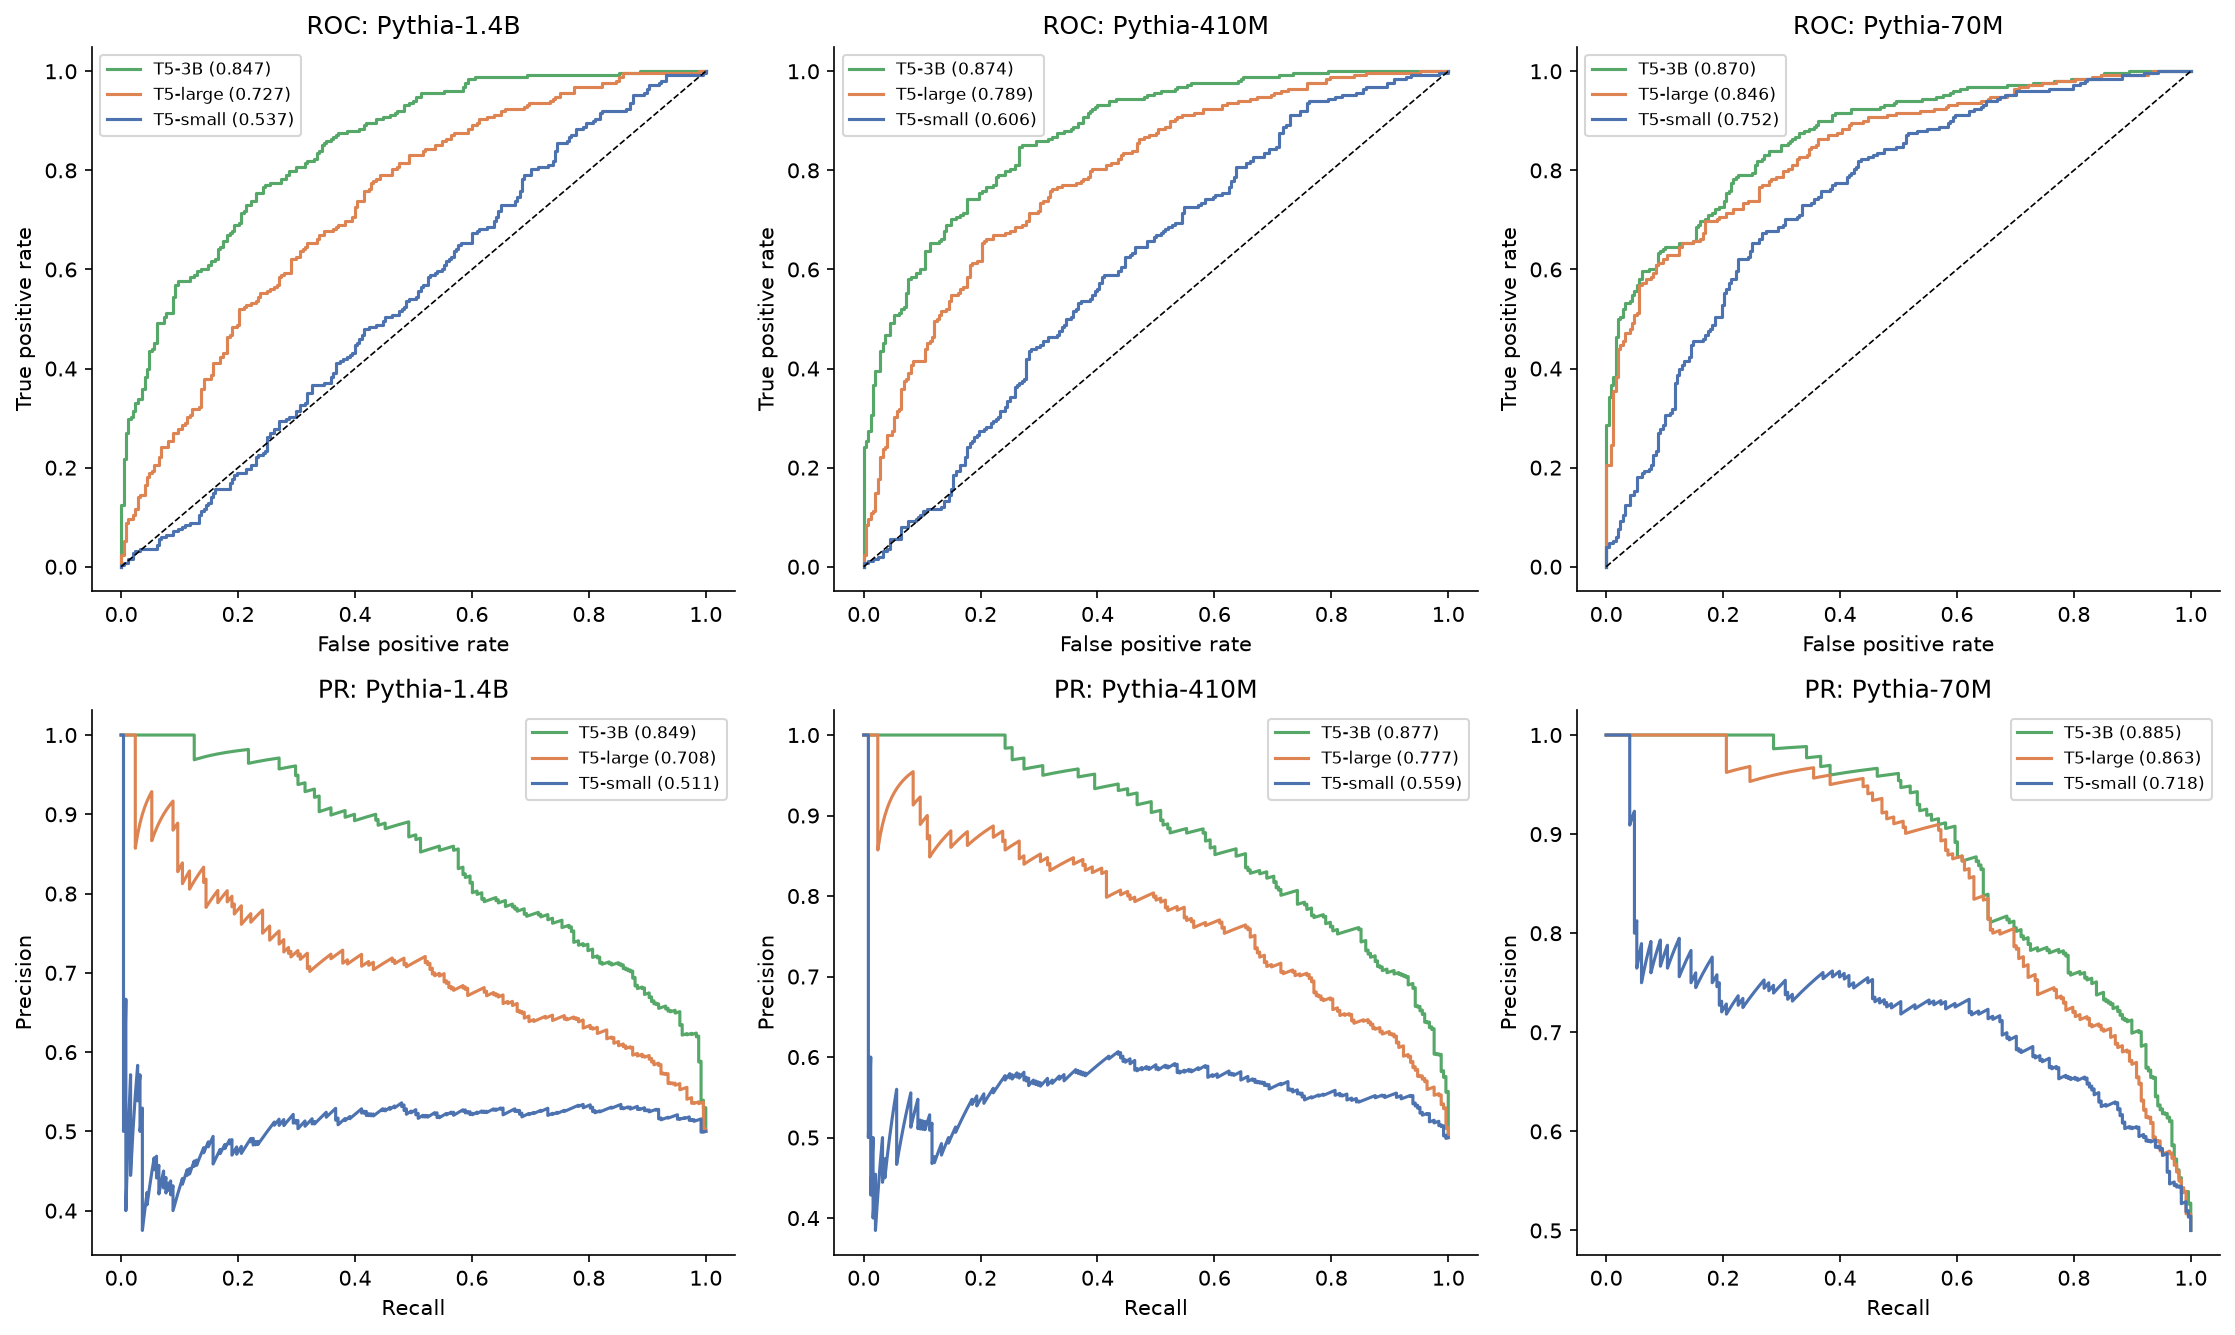
\includegraphics[width=0.6\textwidth]{figures/Experiment3/perturbation_scale_curves.png}
\caption{ROC curves (top row) and PR curves (bottom row) for each Pythia detector under the three T5 mask-filling models. The T5-small curves for the large detectors track the chance diagonal, whilst T5-3B sustains high precision across recall, showing that filler capacity governs whether the curvature signal survives.}
\label{fig:exp3_curves}
\end{figure}
The first trend is a monotonic improvement in detection performance with the capacity of the mask-filling model for every detector. Under the T5-small configuration, performance remains modest, with AUROC values of 0.537, 0.606 and 0.752 for Pythia-1.4B, Pythia-410M and Pythia-70M respectively. The move to T5-large raises every detector by a wide margin, and T5-3B delivers the strongest overall performance, with AUROC values of 0.847, 0.874 and 0.870 across the three detectors.
The second trend concerns the interaction with detector scale. The detector hierarchy established in Chapter \ref{chap:exp1} persists when the perturbation model is weak, but narrows as the perturbation model strengthens. With T5-small, Pythia-70M outperforms Pythia-1.4B by 0.215 AUROC. With T5-3B, the same gap shrinks to 0.023, and the hierarchy even inverts marginally, with Pythia-410M exceeding Pythia-70M by 0.004 AUROC, although Pythia-70M retains the highest PR-AUC (0.885 against 0.877).
The aggregate trade-off is made explicit in Figure \ref{fig:exp3_scale_trend}, which plots each detector's performance against mask-filler parameter count on a logarithmic axis. All three curves rise steeply between T5-small and T5-large and flatten between T5-large and T5-3B, making the diminishing returns explicit. For Pythia-1.4B the AUROC rises by 0.190 then by only 0.120, and for Pythia-70M the gain collapses from 0.094 to 0.024. The detector gap is widest under T5-small and narrows as capacity grows, showing that a faithful perturbation removes most of the detector-scale penalty identified in Chapter \ref{chap:exp1}.
\begin{figure}[H]
\centering
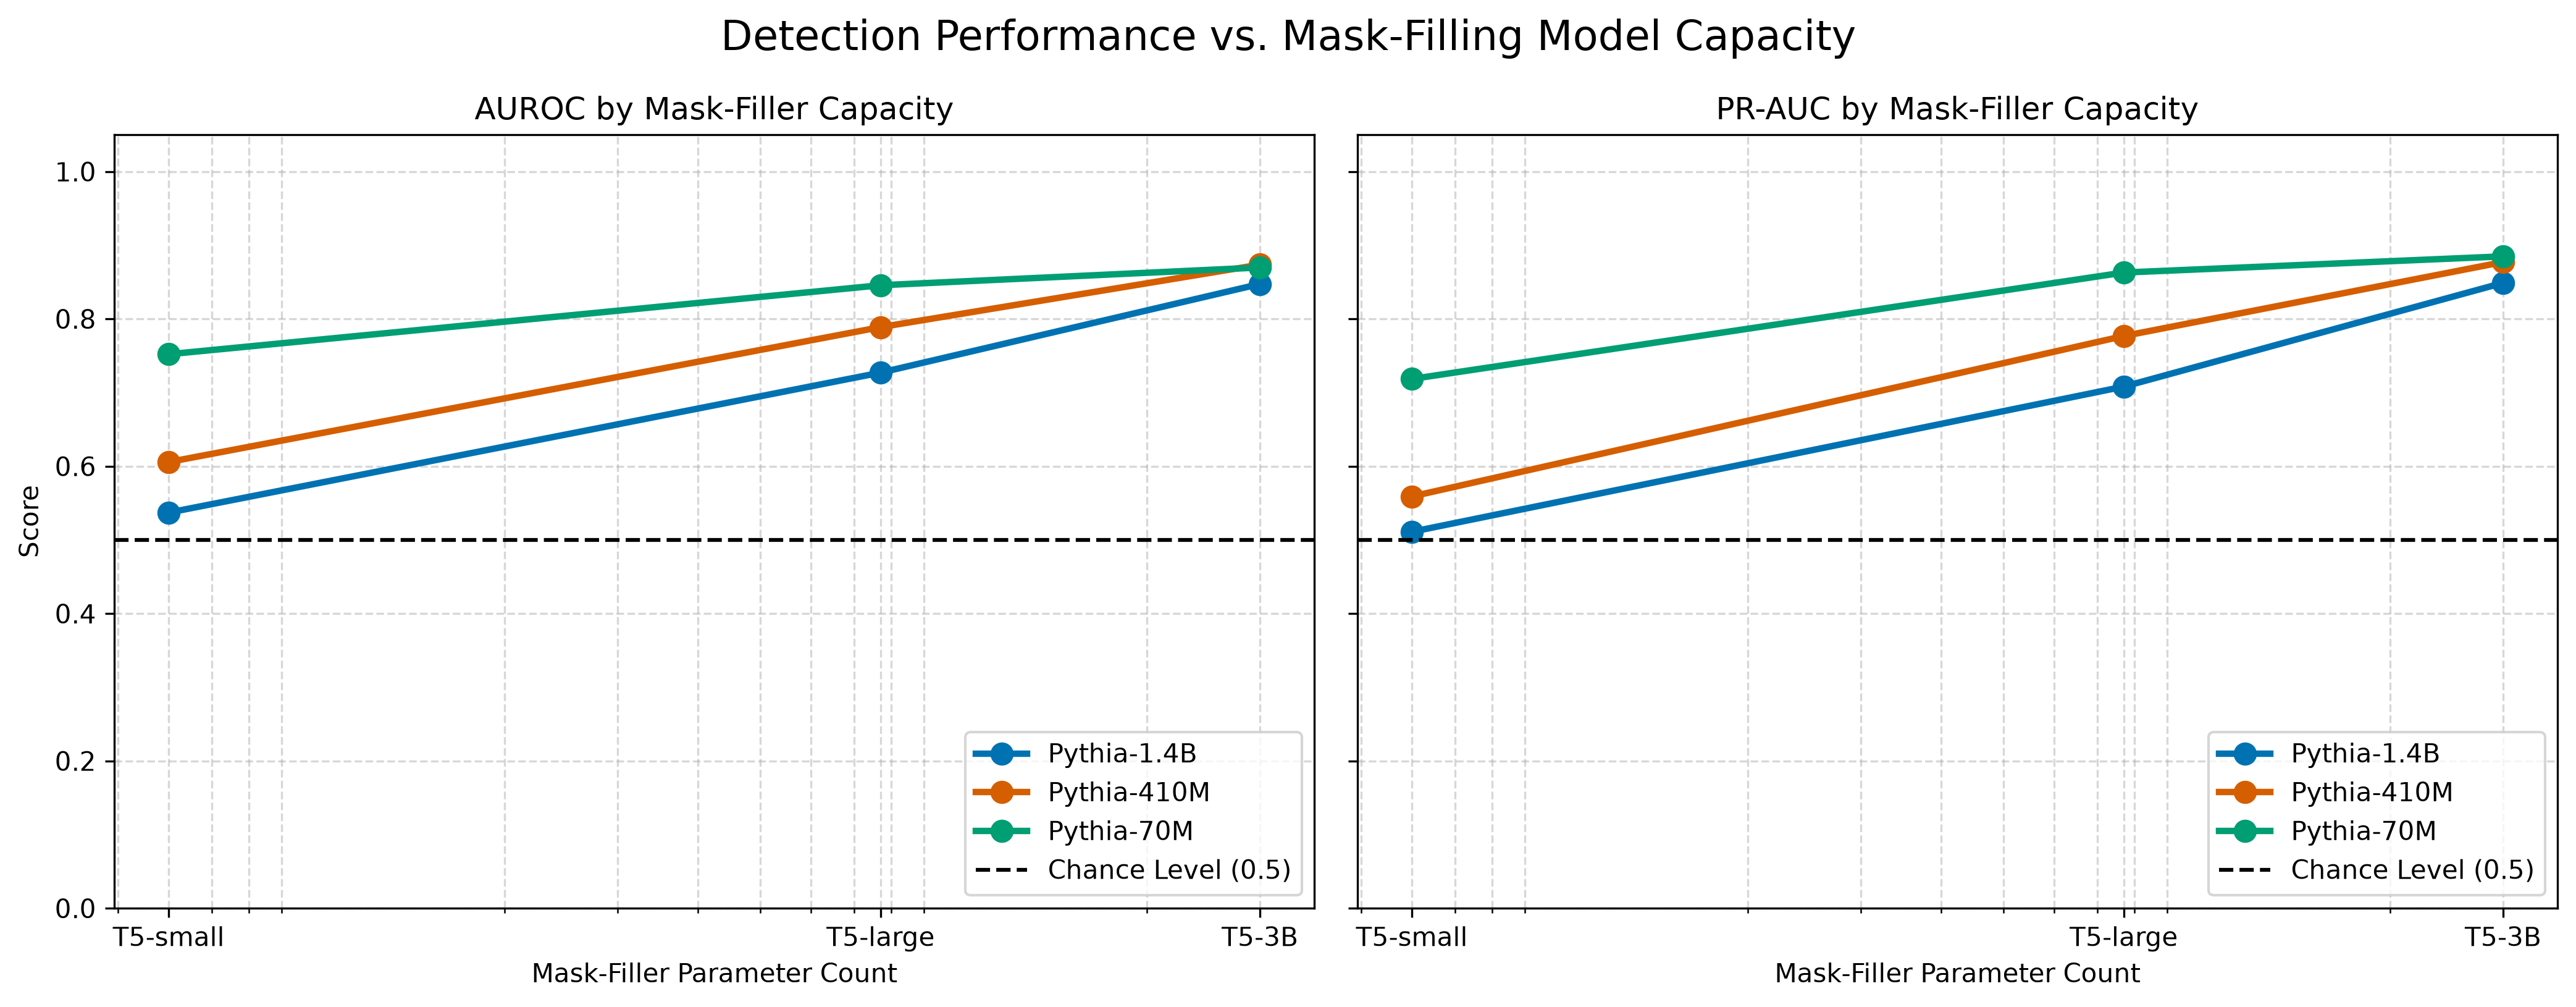
\includegraphics[width=\textwidth]{figures/Experiment3/perturbation_scale_trend.png}
\caption{AUROC (left) and PR-AUC (right) as a function of mask-filling model parameter count for each Pythia detector. All curves rise steeply then flatten, making the diminishing returns explicit, and the detector gap narrows as capacity grows, showing that a faithful perturbation removes most of the detector-scale penalty.}
\label{fig:exp3_scale_trend}
\end{figure}

\section{Mechanistic and Distributional Analysis}
\label{sec:exp3_analysis}
The curvature metric is only as reliable as the neighbourhood that the mask-filling model constructs around each document. A mask-filler must replace the masked spans with tokens that remain plausible within the local context, so that the log probability of each perturbed document reflects the local geometry of the detector likelihood surface rather than the artefacts of a poor reconstruction. Mask-filling fidelity improves with model capacity, as scaling laws, the smooth relationship between size and error reviewed in Chapter \ref{chap:background}, predict for sequence-to-sequence models \citep{kaplan2020scaling, hoffmann2022training}, which is why the neighbourhood quality, and hence the curvature estimate, tracks filler size.
When the mask-filler is too weak, the injected spans drift away from the local context. The perturbed documents then receive low log probabilities for reasons unrelated to the curvature of the original document, and the resulting curvature values become dominated by reconstruction noise, the spurious signal created by a bad fill rather than by the text being judged. The ROC curves for T5-small in Figure \ref{fig:exp3_curves} illustrate this failure mode directly: the curve for Pythia-1.4B tracks the chance diagonal, the line a coin-flip classifier would draw, and the associated PR curve collapses towards the class prior, the 0.5 baseline precision of a balanced dataset, indicating that the reconstruction noise has swallowed the curvature signal entirely.
The interaction with detector scale follows from the findings of Chapter \ref{chap:exp1}. Large detectors possess smooth and conservative likelihood surfaces, so the curvature signal they produce is already weak when the perturbations are faithful, and noisy perturbations erase the signal completely. This explains why Pythia-1.4B suffers the largest penalty under T5-small. Smaller detectors exhibit steeper probability gradients, so even imperfect perturbations produce a usable separation between human and machine text, which is why Pythia-70M remains usable at 0.752 AUROC even with the weakest mask-filler.
As the mask-filler strengthens, the perturbations become faithful local neighbours, and the curvature metric recovers the true local geometry of the likelihood surface. The separation between human and machine text then depends primarily on the intrinsic sharpness of the detector surface, which explains why the detector hierarchy narrows under T5-3B: once the perturbation is no longer the bottleneck, all three detectors recover a meaningful signal and the remaining differences are small.

\section{Discussion and Summary}
\label{sec:exp3_summary}
This experiment demonstrates that the capacity of the mask-filling model is a first-order determinant of curvature-based detection performance. Detection performance increases monotonically from T5-small to T5-3B for every detector, and a weak mask-filler can nullify detection entirely when paired with a large detector, as shown by the near-chance performance of Pythia-1.4B under T5-small.
The results also carry a practical message for edge deployment. The improvement from T5-large to T5-3B is subject to clear diminishing returns, and the pairing of T5-large with Pythia-70M attains 0.846 AUROC and 0.863 PR-AUC, within 0.024 AUROC of the strongest configuration examined. A small detector paired with a medium mask-filler therefore recovers most of the available detection signal at a fraction of the computational cost of the T5-3B configuration.
Two scope boundaries qualify this chapter. The generator is fixed to SmolLM2-1.7B, so the interaction between generator strength and filler capacity is not characterised, and the detector suite is restricted to the Pythia trio. One open question remains: the T5 models compared here all produce semantically coherent infills, fills that preserve the meaning of the sentence, so whether semantic coherence is required at all is not yet established. Chapter \ref{chap:exp4} addresses this question directly by replacing the neural mask-filler with cheaper non-semantic perturbations, namely synonym substitution, unigram frequency sampling and random token insertion, to identify the minimum linguistic prerequisites under which the curvature metric remains effective.

\chapter{Experiment 4: Linguistic Perturbation Strategies}
\label{chap:exp4}
This chapter asks the final question of the comparative analysis: does the perturbation need to mean anything at all? The canonical pipeline spends most of its perturbation budget on semantically coherent infills, that is, fills that preserve the meaning of the sentence, and Experiment 3 confirmed that coherent infills from a strong filler support the curvature signal. The results here overturn the assumption that coherence is the active ingredient: performance follows a pronounced V-shape across the spectrum of linguistic structure, dropping sharply when meaning is preserved but lexical choices are disrupted, and recovering to or above the semantic control once the perturbations become purely statistical. This chapter quantifies that profile and explains why the curvature metric is a statistical probe rather than a semantic comparison.

\section{Experimental Setup}
\label{sec:exp4_setup}
The fourth experiment evaluates the linguistic perturbation strategy as the final manipulated constituent. The generator is fixed to SmolLM2-1.7B \citep{allal2024smollm}, the model that wrote the machine text and the strongest generator identified in Chapter \ref{chap:exp1}, and the detector suite comprises the three Pythia models at their released checkpoints, matching the configuration of Chapter \ref{chap:exp3}. The evaluation again uses 250 human-written and 250 machine-generated samples, with 30\% of tokens masked in spans of length two (pairs of consecutive words are hidden) and 50 perturbed variants (edited copies) drawn per sample.
Four strategies span the spectrum from full semantic coherence to pure token noise. The semantic control refills the masks with the T5-large mask-filler, the reference configuration selected in Chapter \ref{chap:exp3}, in which a neural model rewrites the blanks so the sentence keeps its meaning. The synonym strategy replaces masked spans with lexical substitutes drawn from WordNet \citep{miller1995wordnet}, a lexical database that lists the synonyms of a word, preserving local meaning whilst disrupting the original lexical choices. The random words strategy samples substitutes according to unigram frequency, how often each word appears in the corpus, retaining global lexical statistics but removing contextual coherence. The random tokens strategy inserts uniformly sampled vocabulary tokens, removing both semantic content and lexical plausibility. Table \ref{tab:perturbation_example} shows the four strategies applied to the same document.

\section{Quantitative Results}
\label{sec:exp4_results}
Figure \ref{fig:exp4_bars} reports AUROC and PR-AUC per detector and strategy, Figure \ref{fig:exp4_lines} traces the progression across strategies, and Figure \ref{fig:exp4_curves} shows the ROC and PR curves. The central finding is a pronounced V-shaped relationship between linguistic structure and detection efficacy.
\begin{figure}[H]
\centering
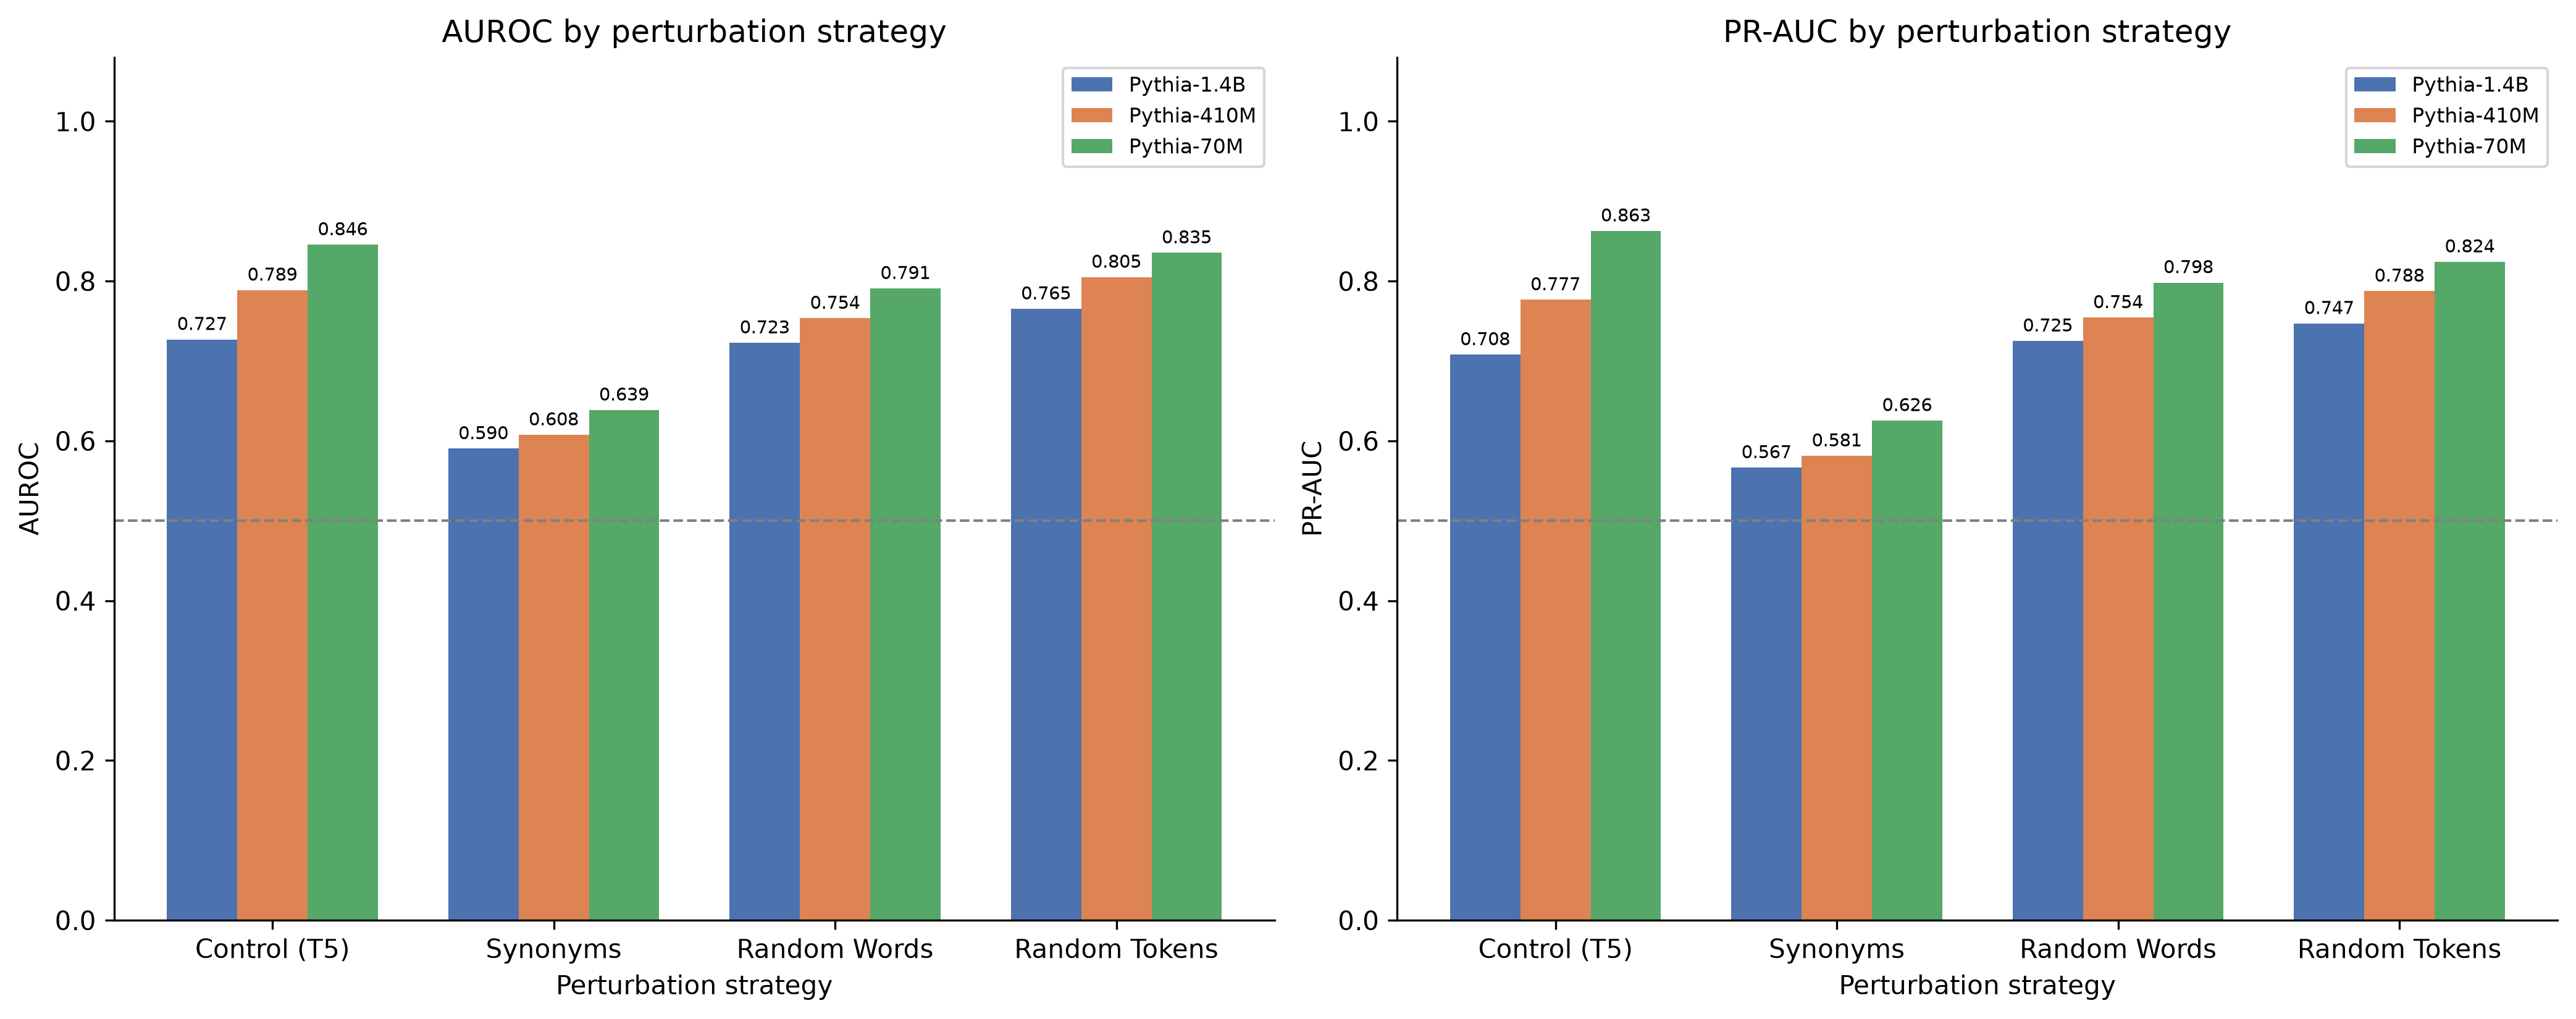
\includegraphics[width=\textwidth]{figures/Experiment4/exp4_strategy_bars.png}
\caption{AUROC and PR-AUC for each perturbation strategy across the three Pythia detectors, with the generator fixed to SmolLM2-1.7B. Synonym substitution collapses every detector towards the dashed chance line, whilst random words and random tokens recover or exceed the semantic control, showing that statistical disruption suffices.}
\label{fig:exp4_bars}
\end{figure}
\begin{figure}[H]
\centering
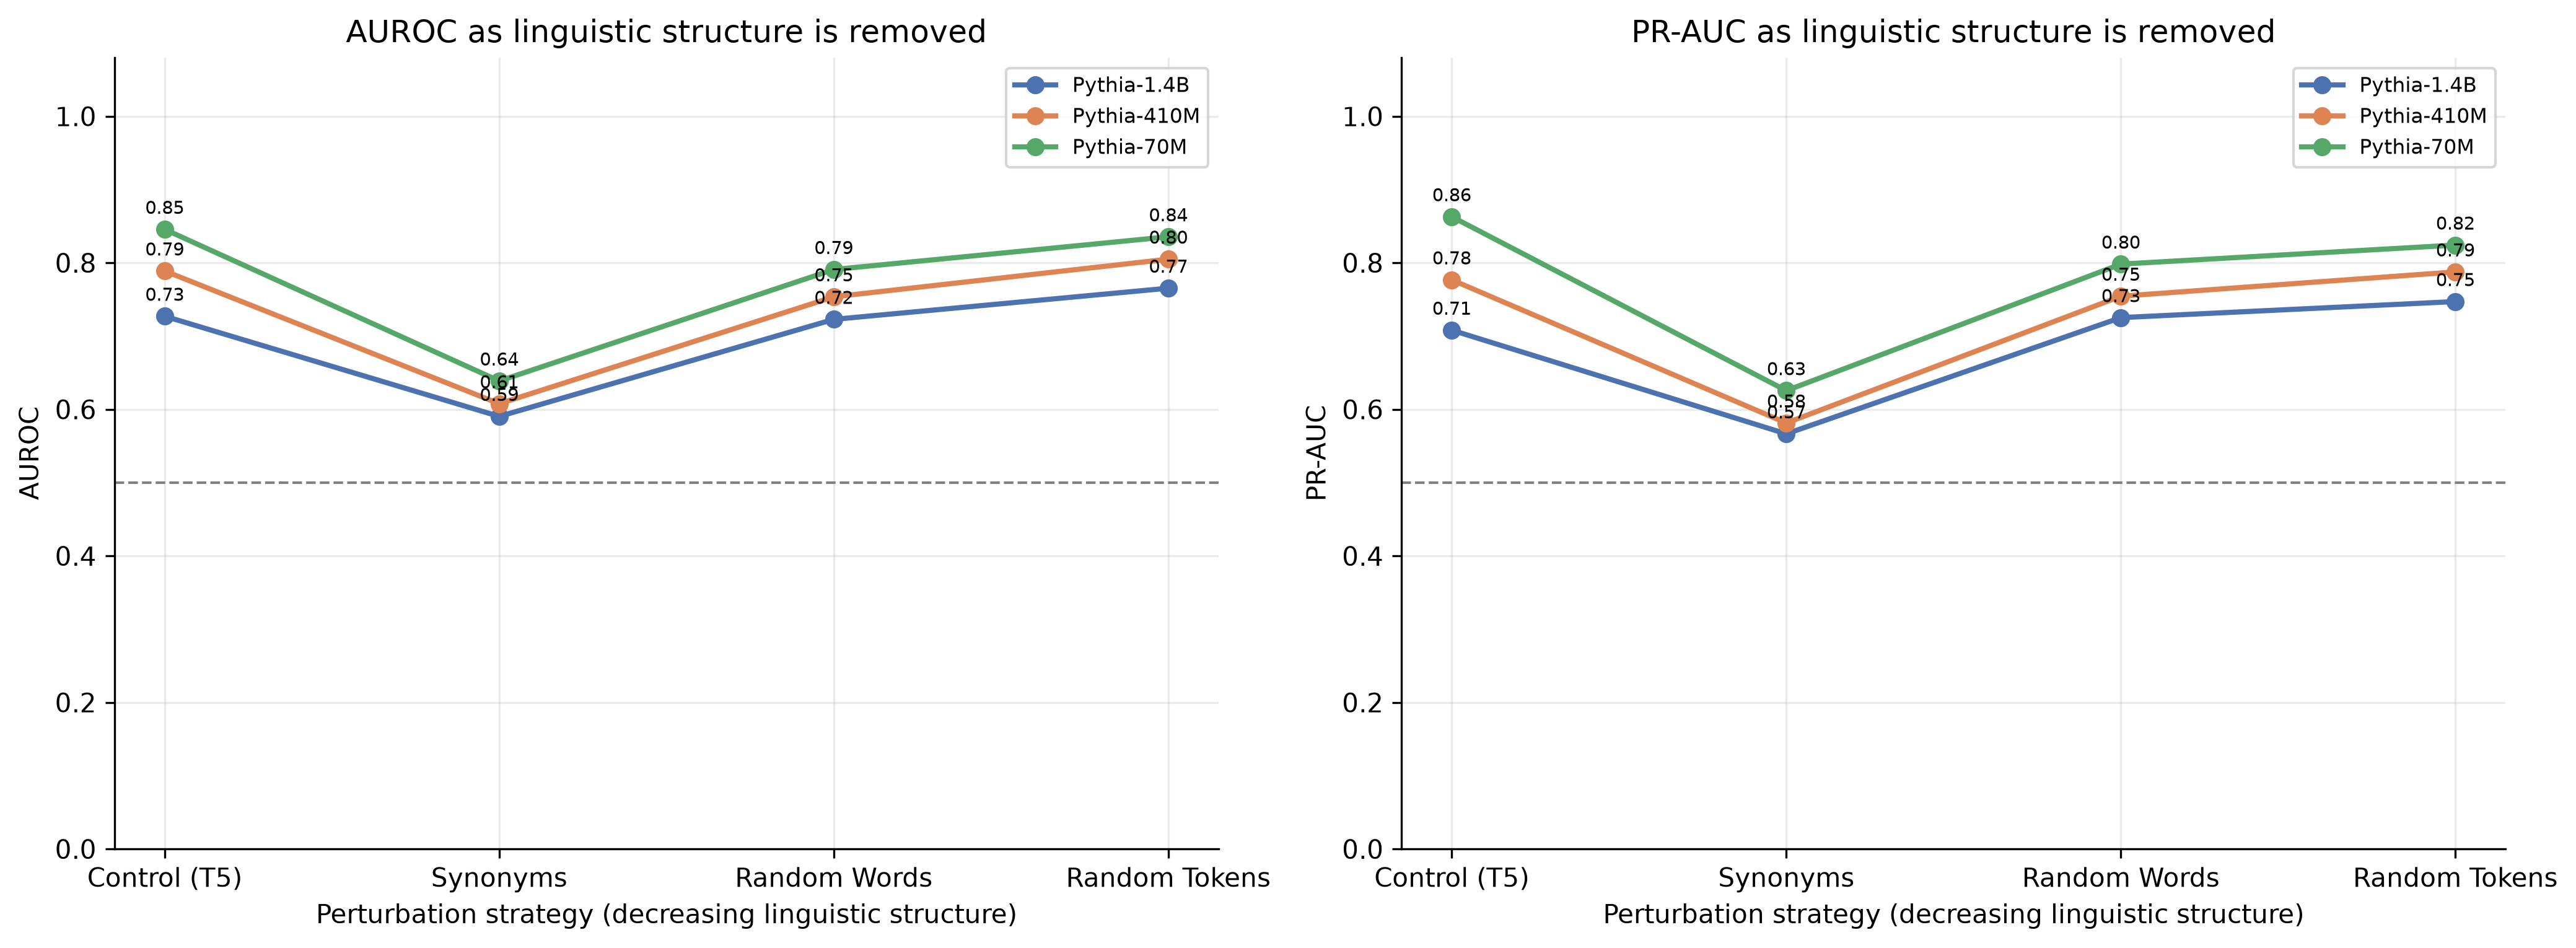
\includegraphics[width=\textwidth]{figures/Experiment4/exp4_degradation_lines.png}
\caption{Progression of AUROC and PR-AUC across the four perturbation strategies for each Pythia detector, ordered from full semantic coherence to pure token noise. All three detectors trace the same V-shape, with the dip at synonyms and the recovery under statistical perturbations.}
\label{fig:exp4_lines}
\end{figure}
\begin{figure}[H]
\centering
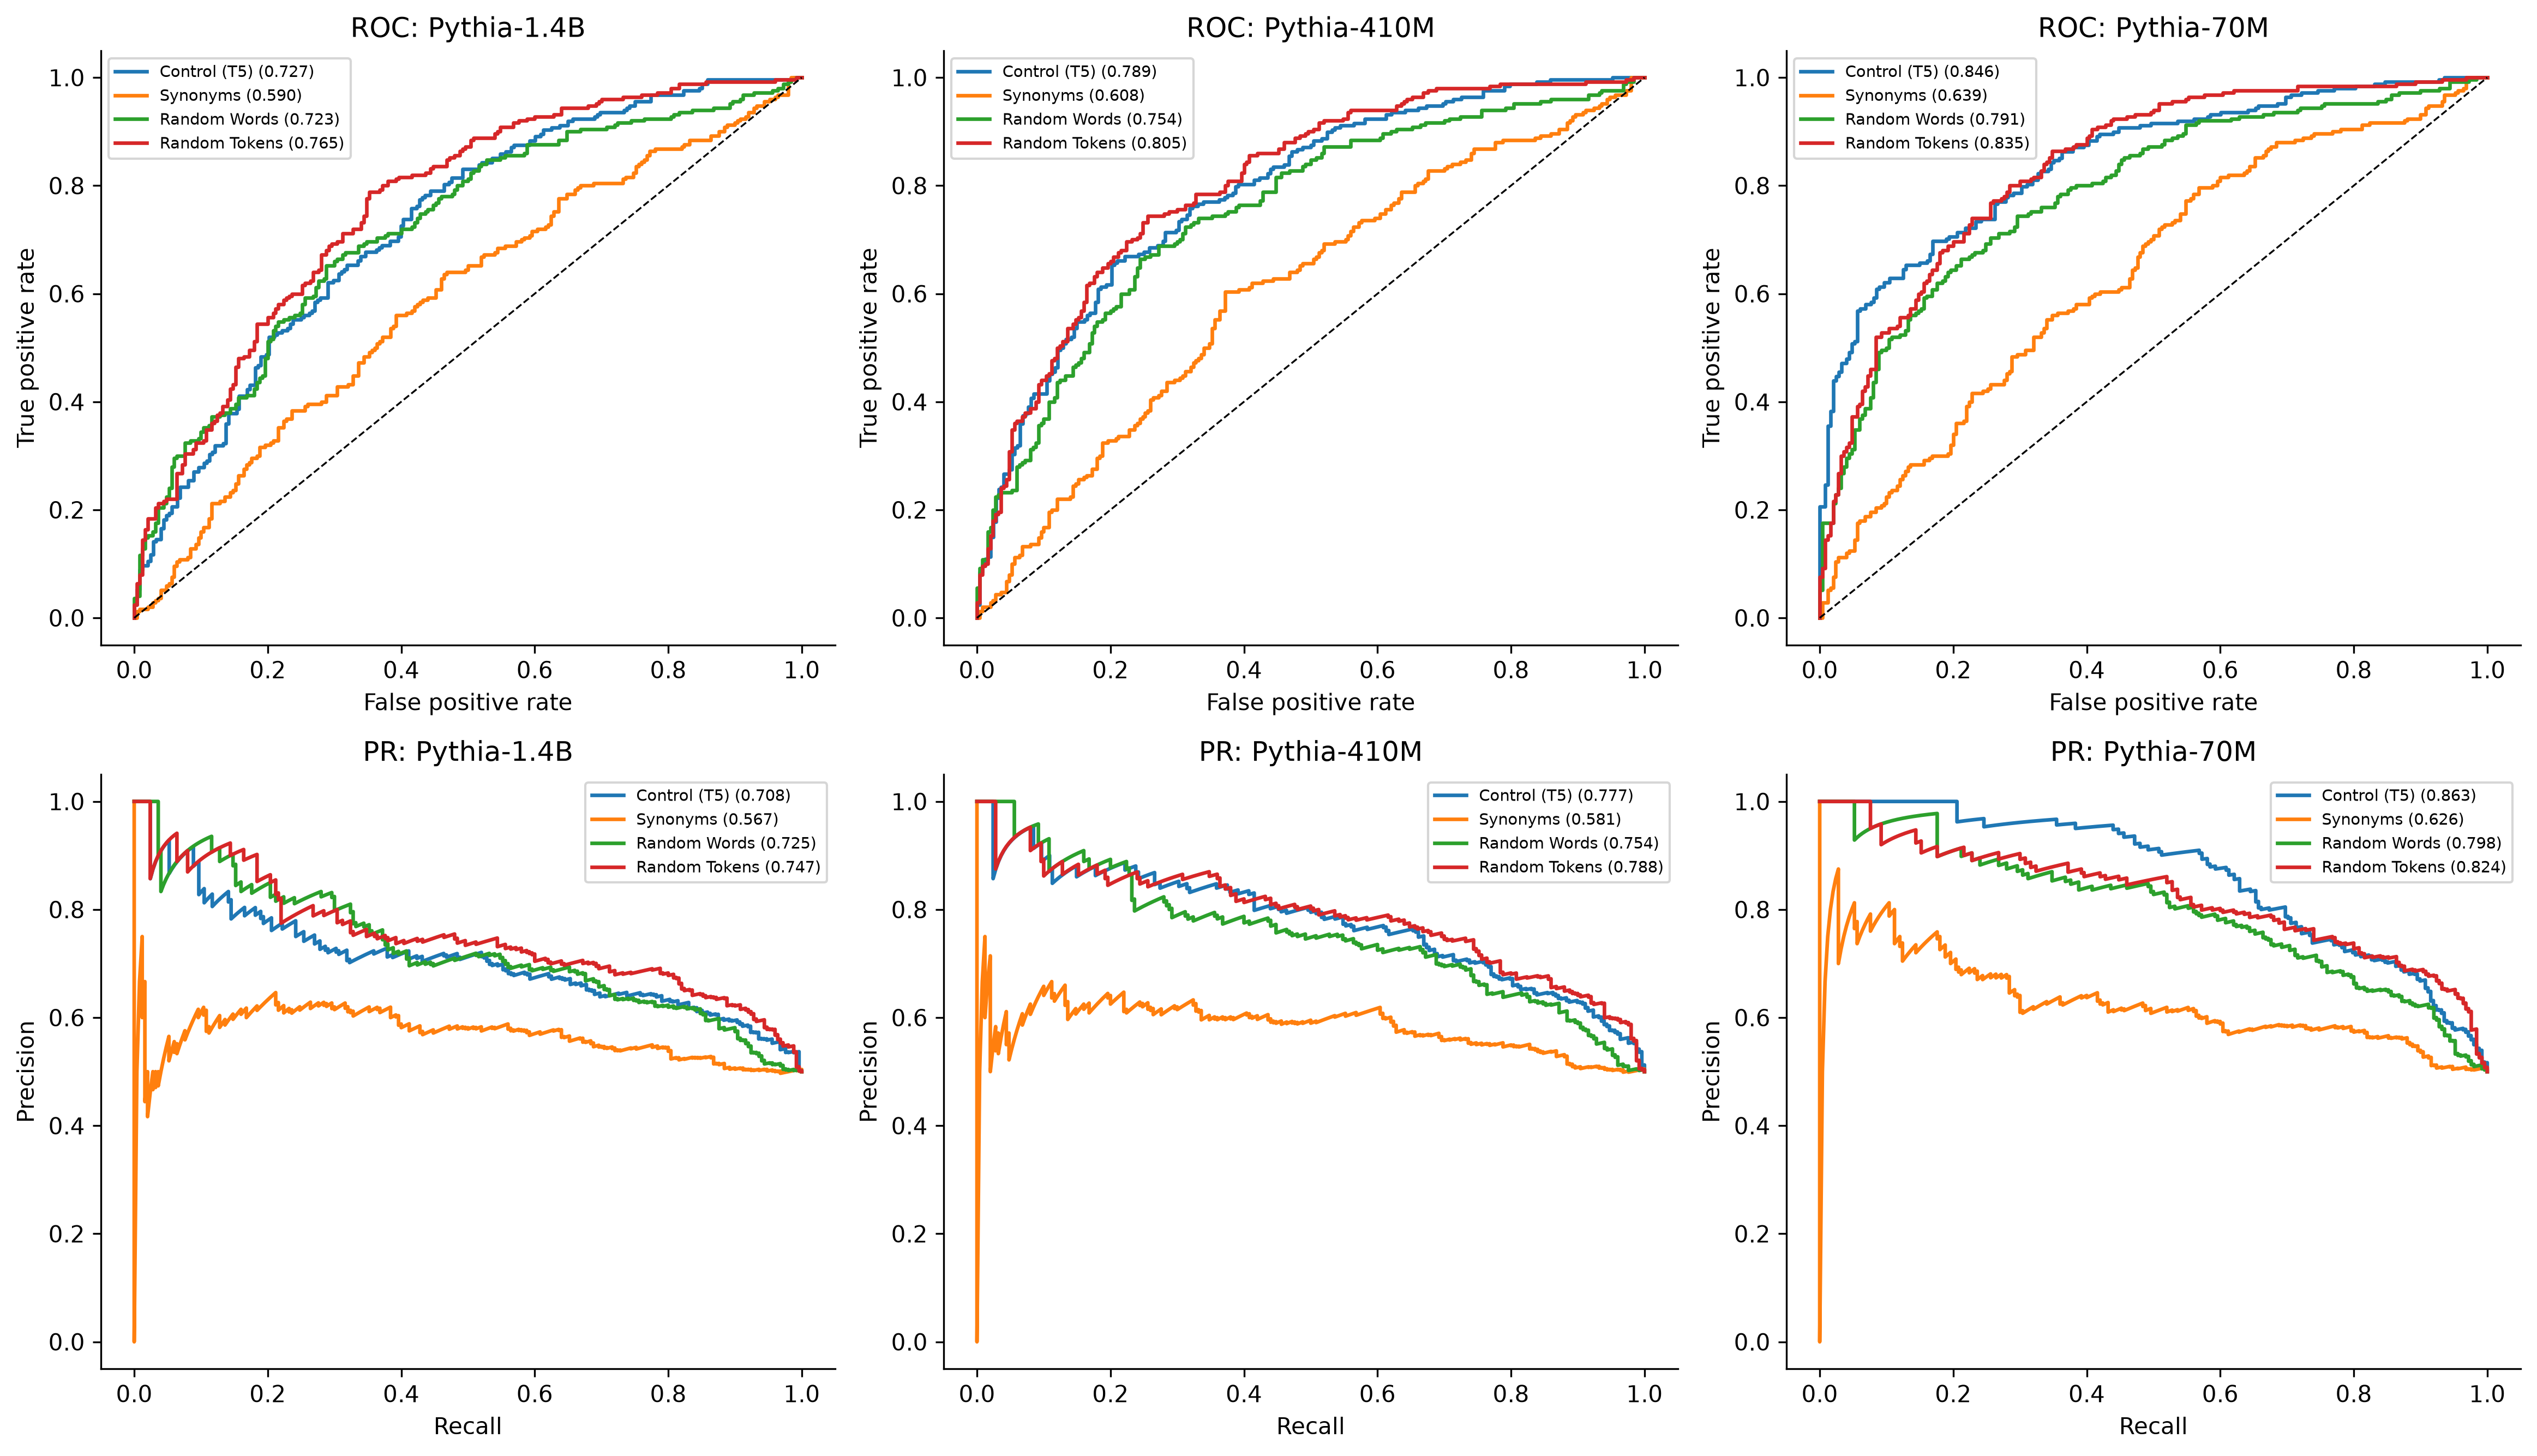
\includegraphics[width=\textwidth]{figures/Experiment4/exp4_roc_pr_curves.png}
\caption{ROC curves (top row) and PR curves (bottom row) for each Pythia detector under the four perturbation strategies. The synonym curves track the chance diagonal whilst the statistical strategies match or exceed the semantic control, confirming that the curvature signal survives without semantic coherence.}
\label{fig:exp4_curves}
\end{figure}
Under the semantic control, the Pythia detectors achieve AUROC scores of 0.727, 0.789 and 0.846 for the 1.4B, 410M and 70M models respectively. Substitution of the neural infiller with WordNet synonyms degrades every detector, reducing AUROC to 0.590, 0.608 and 0.639, only marginally above the coin-flip level of 0.5. Removal of semantic coherence altogether restores detection efficacy. The random words strategy recovers AUROC scores of 0.723, 0.754 and 0.791, closely matching the control, and the random tokens strategy matches or exceeds the control for the two larger detectors, reaching 0.765 for Pythia-1.4B and 0.805 for Pythia-410M. Only the smallest detector retains a clear advantage for the semantic control, with the control achieving 0.846 AUROC and 0.863 PR-AUC against 0.835 and 0.824 for random tokens.
The PR-AUC results in Figure \ref{fig:exp4_bars} exhibit the same profile, with the synonym condition collapsing to 0.567, 0.581 and 0.626 across the three detectors. The detector hierarchy established in Chapter \ref{chap:exp1} persists across every strategy, but its magnitude narrows under synonym substitution, where all detectors perform poorly, and is most pronounced under the statistically driven strategies.
The aggregate profile is made explicit in Figure \ref{fig:exp4_trend}, which averages performance over the three detectors. Mean AUROC falls from roughly 0.79 under the semantic control to 0.61 under synonyms, then recovers to 0.76 under random words and 0.80 under random tokens, so the statistically driven perturbations match or exceed the coherent control. The PR-AUC panel shows the same V-shape.
\begin{figure}[H]
\centering
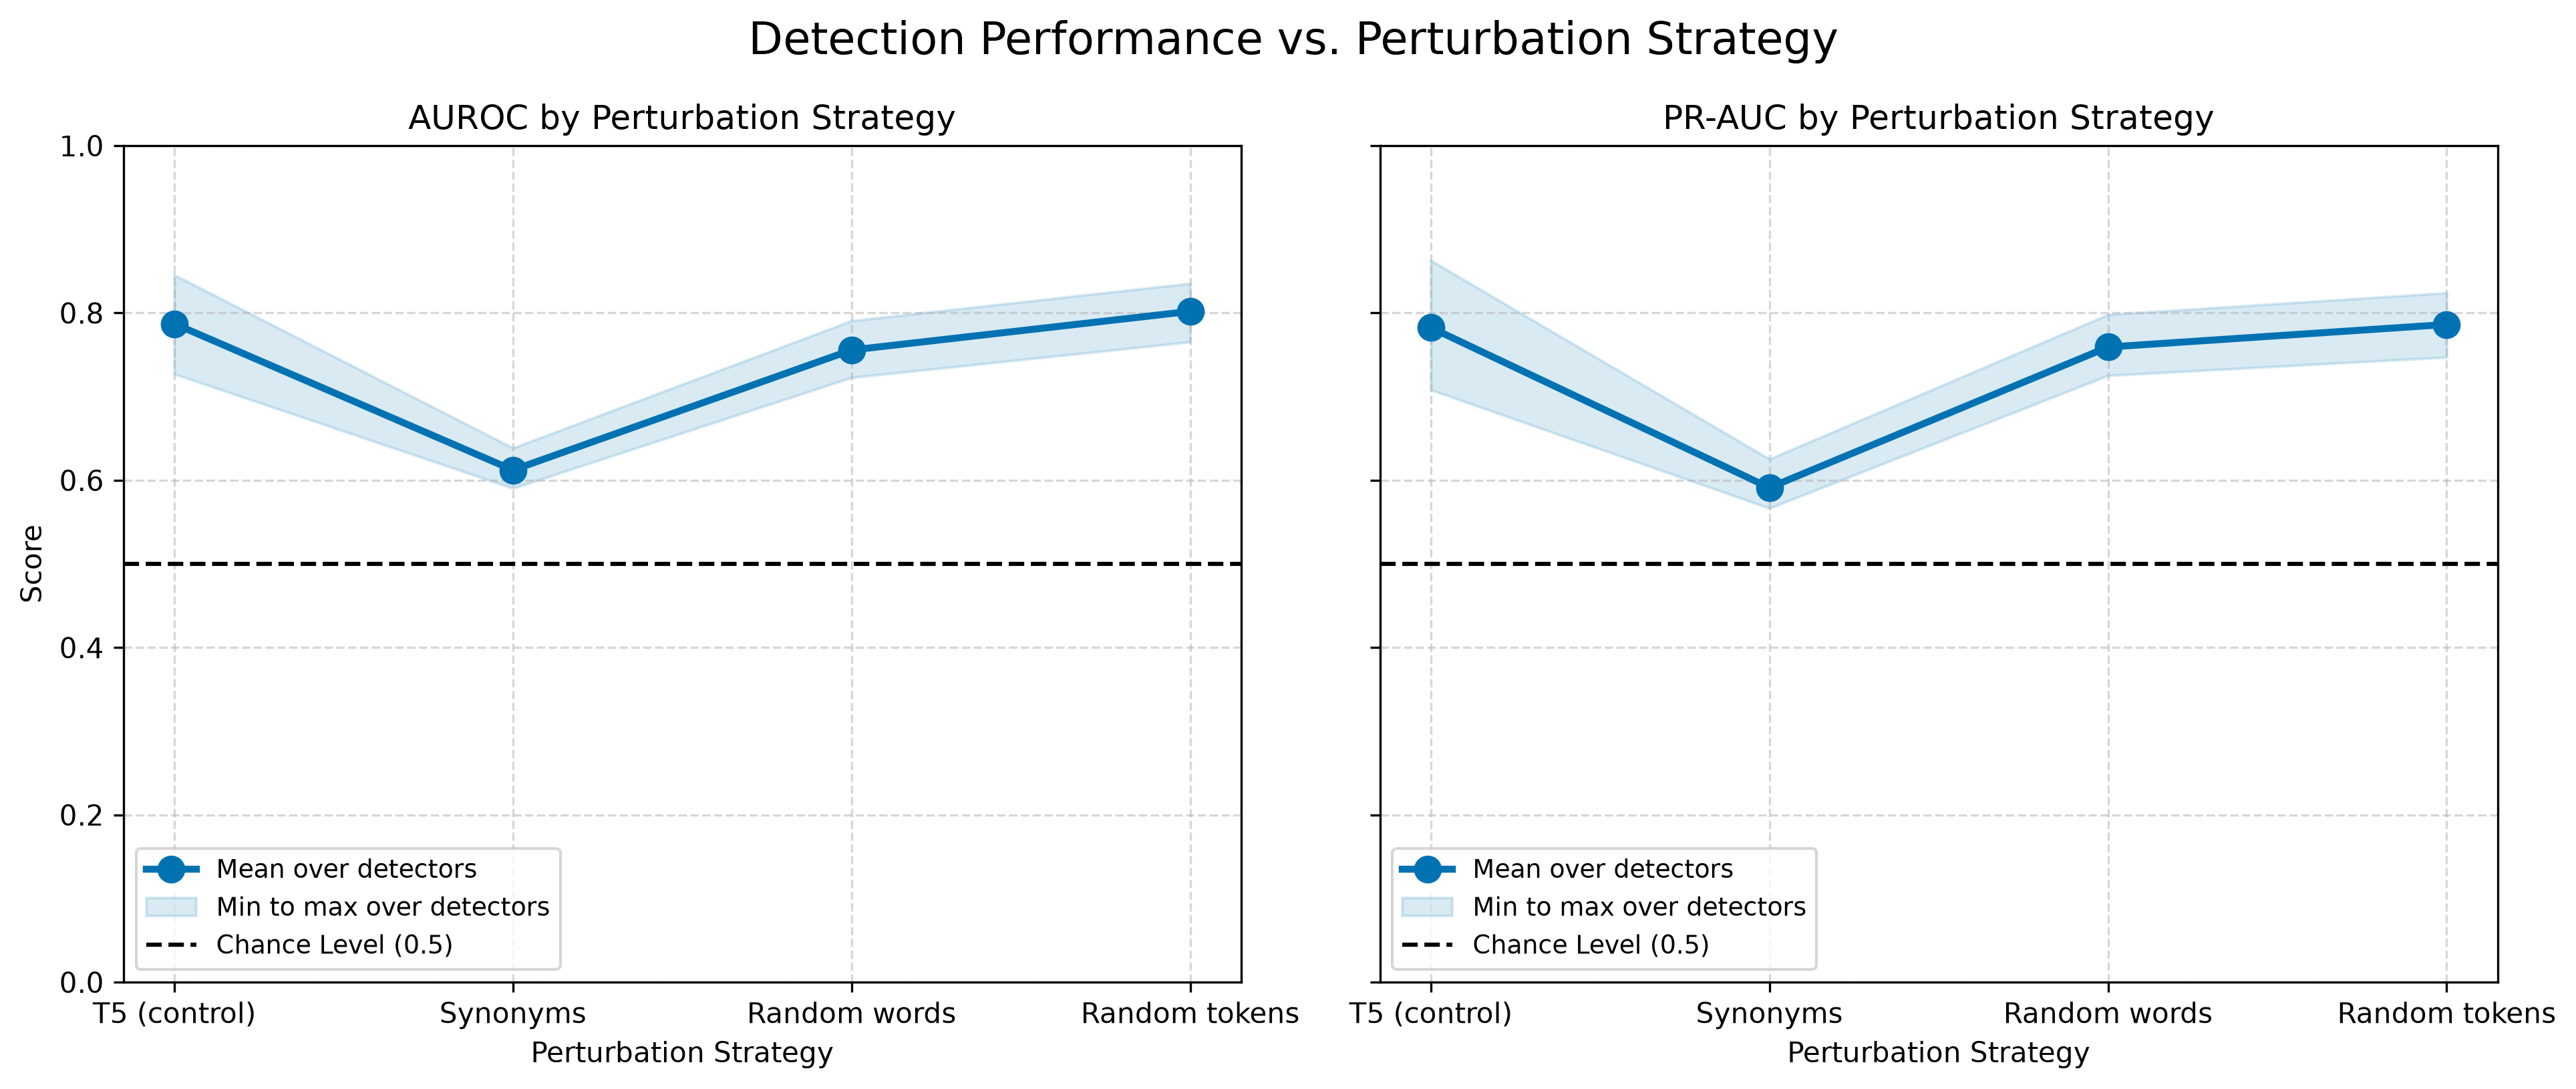
\includegraphics[width=\textwidth]{figures/Experiment4/exp4_strategy_trend.png}
\caption{Mean AUROC (left) and PR-AUC (right) by perturbation strategy, averaged across the three Pythia detectors, with the shaded band showing the min-to-max spread over detectors. Performance drops sharply under synonym substitution and recovers to or above the semantic control under statistically driven perturbations, showing that semantic coherence is not required for an effective curvature signal.}
\label{fig:exp4_trend}
\end{figure}

\section{Mechanistic and Distributional Analysis}
\label{sec:exp4_analysis}
The V-shape demonstrates that the curvature metric probes local likelihood sharpness, not semantics. Semantic coherence in the perturbation is not a prerequisite; in several configurations pure token noise outperforms the coherent control.
Synonym substitution preserves the meaning of the sentence whilst introducing statistically atypical substitutes. For machine text, which sits in a narrow, overconfident region of the detector surface, meaning-preserving substitutes keep the perturbed neighbours close to the generator's own sampling region and attenuate the drop in log probability. For human text, the atypical substitutes disrupt natural collocations, words that habitually appear together, and increase the drop. The curvature gap therefore narrows and discrimination collapses towards chance, as the near-diagonal synonym ROC curves in Figure \ref{fig:exp4_curves} show. This is consistent with the broader observation that semantic-preserving transformations, such as paraphrasing, are precisely the transformations that most weaken statistical detection signals \citep{sadasivan2023can}.
Random words and random tokens act as distribution-free disruptions, edits that make no attempt to imitate real text. They push machine text far outside its narrow sampling region, producing a large and consistent drop in log probability, whilst human text, which occupies a broader region of the surface, absorbs the disruption with a smaller relative drop. The separation is therefore preserved and efficacy recovers to the control level. The account also explains why detection can rest on purely statistical cues: the literature on statistical fingerprints of synthetic text reaches the same conclusion \citep{uchendu2021turingbench}, and Fast-DetectGPT's sampling-based perturbations likewise dispense with semantic infilling \citep{bao2024fast}.
The benefit of random perturbations is largest for the largest detector, consistent with the smoother surfaces identified in Chapter \ref{chap:exp1}: conservative detectors require stronger statistical disruption to expose the sharpness of their surfaces. Only the smallest detector, Pythia-70M, retains a clear advantage for the semantic control, because its steep gradients already extract a strong signal from coherent neighbours.

\newpage
\section{Discussion and Summary}
\label{sec:exp4_summary}
This experiment establishes that the curvature metric does not require semantically coherent perturbations. WordNet synonym substitution, despite preserving meaning, yields the weakest performance of all four strategies, whilst statistically driven perturbations match or exceed the semantic control and surpass it outright for the larger detectors. The curvature metric is therefore best understood as a statistical probe of local likelihood sharpness, and the computational expense of neural mask-filling is not a prerequisite for effective detection.
The result completes the compression of the pipeline. Replacement of the neural infiller with uniform random token substitution removes the most expensive component of the perturbation phase, reducing the pipeline to a small detector and an inexpensive random substitution. Together with the small, partially trained detectors of Chapters \ref{chap:exp1} and \ref{chap:exp2}, this yields a fully lightweight, architecture-agnostic detector suitable for consumer hardware. The comparative analysis therefore concludes that detection efficacy is driven by the statistical sharpness of the detector surface and the statistical strength of the perturbation, rather than by model size, training convergence, perturbation capacity or semantic fidelity.
Two scope boundaries qualify this chapter. The generator is fixed to SmolLM2-1.7B and the detector suite to the Pythia trio, so the strategy comparison is not repeated across the full cross-detection matrix of Chapter \ref{chap:exp1}, and the masking ratio and span length are held fixed. Chapter \ref{chap:conclusion} synthesises the four experiments, assesses the practical viability of edge deployment, and states the limitations and future work.

\chapter{Conclusion}
\label{chap:conclusion}
This dissertation has raised a single practical question: can curvature-based detection of machine-generated text be executed within the computational constraints of consumer hardware? The four experiments yielded an affirmative answer, but only because the computational weight of the canonical pipeline is an artefact of its instantiation rather than of the method itself. Detection efficacy is driven by the statistical sharpness of the detector likelihood surface and the statistical strength of the perturbation, not by parameter count, training convergence, filler capacity or semantic fidelity. The cheapest correct instantiation, a small partially trained detector paired with random token substitution, is therefore, among the strongest.

\section{Synthesis of Findings}
\label{sec:synthesis}
Chapter \ref{chap:exp1} showed that detector efficacy is inversely related to parameter count: Pythia-70M and DistilGPT-2 exceed 0.90 on AUROC, the probability that a randomly drawn machine document outscores a randomly drawn human document, against the majority of 13 unseen generators, whilst the largest detectors fall to random chance. Chapter \ref{chap:exp2} showed that the same sensitivity is a function of training state: all three Pythia scales start near 0.94 mean AUROC at 1k steps, the decline to 143k steps grows with parameter count, and the optimal window lies between 1,000 and 10,000 steps, meaning the best detectors are partially trained checkpoints, saved copies of the weights taken before convergence. Chapter \ref{chap:exp3} showed that mask-filler capacity, the size of the model that rewrites the masked blanks, governs perturbation fidelity, with monotonic gains from T5-small to T5-3B but diminishing returns beyond T5-large. Chapter \ref{chap:exp4} showed that semantic coherence is not required at all: synonym substitution collapses every detector towards chance, whilst random words and random tokens match or exceed the semantic control, the T5-large configuration in which a neural model rewrites the masks.
Taken together, these results support a single mechanistic account. Machine-generated text resides in narrow, overconfident minima of the detector likelihood surface, so any perturbation, any small edit, that displaces it produces a large and consistent drop in log probability, whilst human text absorbs the same disruption with a smaller relative drop. Small and partially trained detectors expose the sharpest gradients and therefore the largest separation, and statistically strong perturbations are sufficient to probe that sharpness. The curvature metric is ergo a statistical probe of local likelihood sharpness, not a semantic comparison.

\section{A Viable Edge Configuration}
\label{sec:edge_config}
The practical consequence is a concrete configuration. A 70-million-parameter detector at an early checkpoint occupies only a few hundred megabytes, and random token substitution removes the mask-filling model entirely. The pipeline therefore reduces to one small forward-scoring model and an inexpensive substitution operation, with no labelled data, no generator access and no cloud inference. Within the scope of this dissertation, this configuration satisfies the latency, privacy and bandwidth constraints that preclude large detectors from real-time monitoring on edge devices, consumer products such as phones, browser extensions and embedded boards, and it removes the two dominant computational bottlenecks of prior work, namely the large scoring model and the large mask-filling model.

\section{Limitations}
\label{sec:limitations}
Several limitations constrain the generalisability of these findings:
\begin{itemize}
\item \textbf{Zero-shot only.} No supervised fine-tuning was performed, which preserves the architecture-agnostic, training-free character of the method but means the results characterise zero-shot capability rather than an upper bound.
\item \textbf{Single corpus and language.} The evaluation used the WritingPrompts corpus in English, so the findings may not transfer to other registers or languages.
\item \textbf{Restricted generator suite.} Only open, decoder-only Transformers were used, and newer or proprietary generators might have exhibit different likelihood geometries.
\item \textbf{Fixed perturbation hyperparameters.} The masking ratio (30\% of tokens in spans of length two, 50 variants) was held constant, and the sensitivity of the findings to these choices was unexamined.
\item \textbf{No adversarial post-processing.} Adversarial transformations such as paraphrasing and translation, which might have disrupted the curvature signal in deployment, were not considered.
\item \textbf{No on-hardware measurements.} The viability argument rested on parameter counts and removed bottlenecks; actual latency, memory and energy on edge hardware were not reported.
\end{itemize}

\section{Future Work}
\label{sec:future_work}
Future research can extend this work in several directions:
\begin{itemize}
\item \textbf{Broader coverage.} Extend the evaluation to additional domains, languages, and newer or proprietary generators, to test the likelihood-sharpness account beyond open decoder-only architectures.
\item \textbf{Adversarial robustness.} Investigate the interaction between perturbation strategy and adversarial paraphrasing, which may restore the semantic coherence that attenuates the curvature signal.
\item \textbf{Adaptive masking.} Adjust the masking ratio and span length to text length and register, to stabilise the curvature signal.
\item \textbf{Relaxed zero-shot.} Explore lightweight fine-tuning of small detectors, which may sharpen their likelihood surfaces without compromising the edge budget.
\item \textbf{Hybrid signals.} Combine the curvature score with complementary statistical cues, such as token cohesiveness or stylometric features, at negligible additional cost.
\end{itemize}
In sum, this dissertation converts curvature-based detection from a cloud-bound method into one that a consumer device can run, and it identifies the statistical sharpness of the likelihood surface as the variable that makes detection possible.

\bibliographystyle{apa}
\bibliography{mybibfile}

% You may delete everything from \appendix up to \end{document} if you don't need it.
\appendix
\end{document}